\documentclass[pdftex,12pt]{article}

\usepackage[utf8]{inputenc}
\usepackage[english]{babel}
\usepackage[english]{isodate}
\usepackage[parfill]{parskip}
\usepackage[pdftex]{graphicx}
\usepackage{todonotes} % \todo{note} \listoftodos
\usepackage{microtype}
\usepackage{titling}
\usepackage{booktabs}
\usepackage{multirow}
\usepackage{hyperref}
\usepackage{float}
\usepackage{longtable}
\usepackage{tablefootnote}
\usepackage{chngpage}
\usepackage[margin=1in]{geometry}

% Commands
\newcommand{\HRule}{\rule{\linewidth}{0.5mm}}

\title{Maxwell Katz for Dummies}
\author{Harrison J Katz}
\date{\today}

\begin{document}
\pagenumbering{Roman}

% Title Page
\begin{titlepage}
    \begin{center}
        \ % starts a paragraph so tex is happy
        \textsc{\huge \thetitle}\\
        \textsc{An Instruction Manual}\\[1em]
        \HRule \\[1em]

        \begin{figure}[h!]
            \centering
            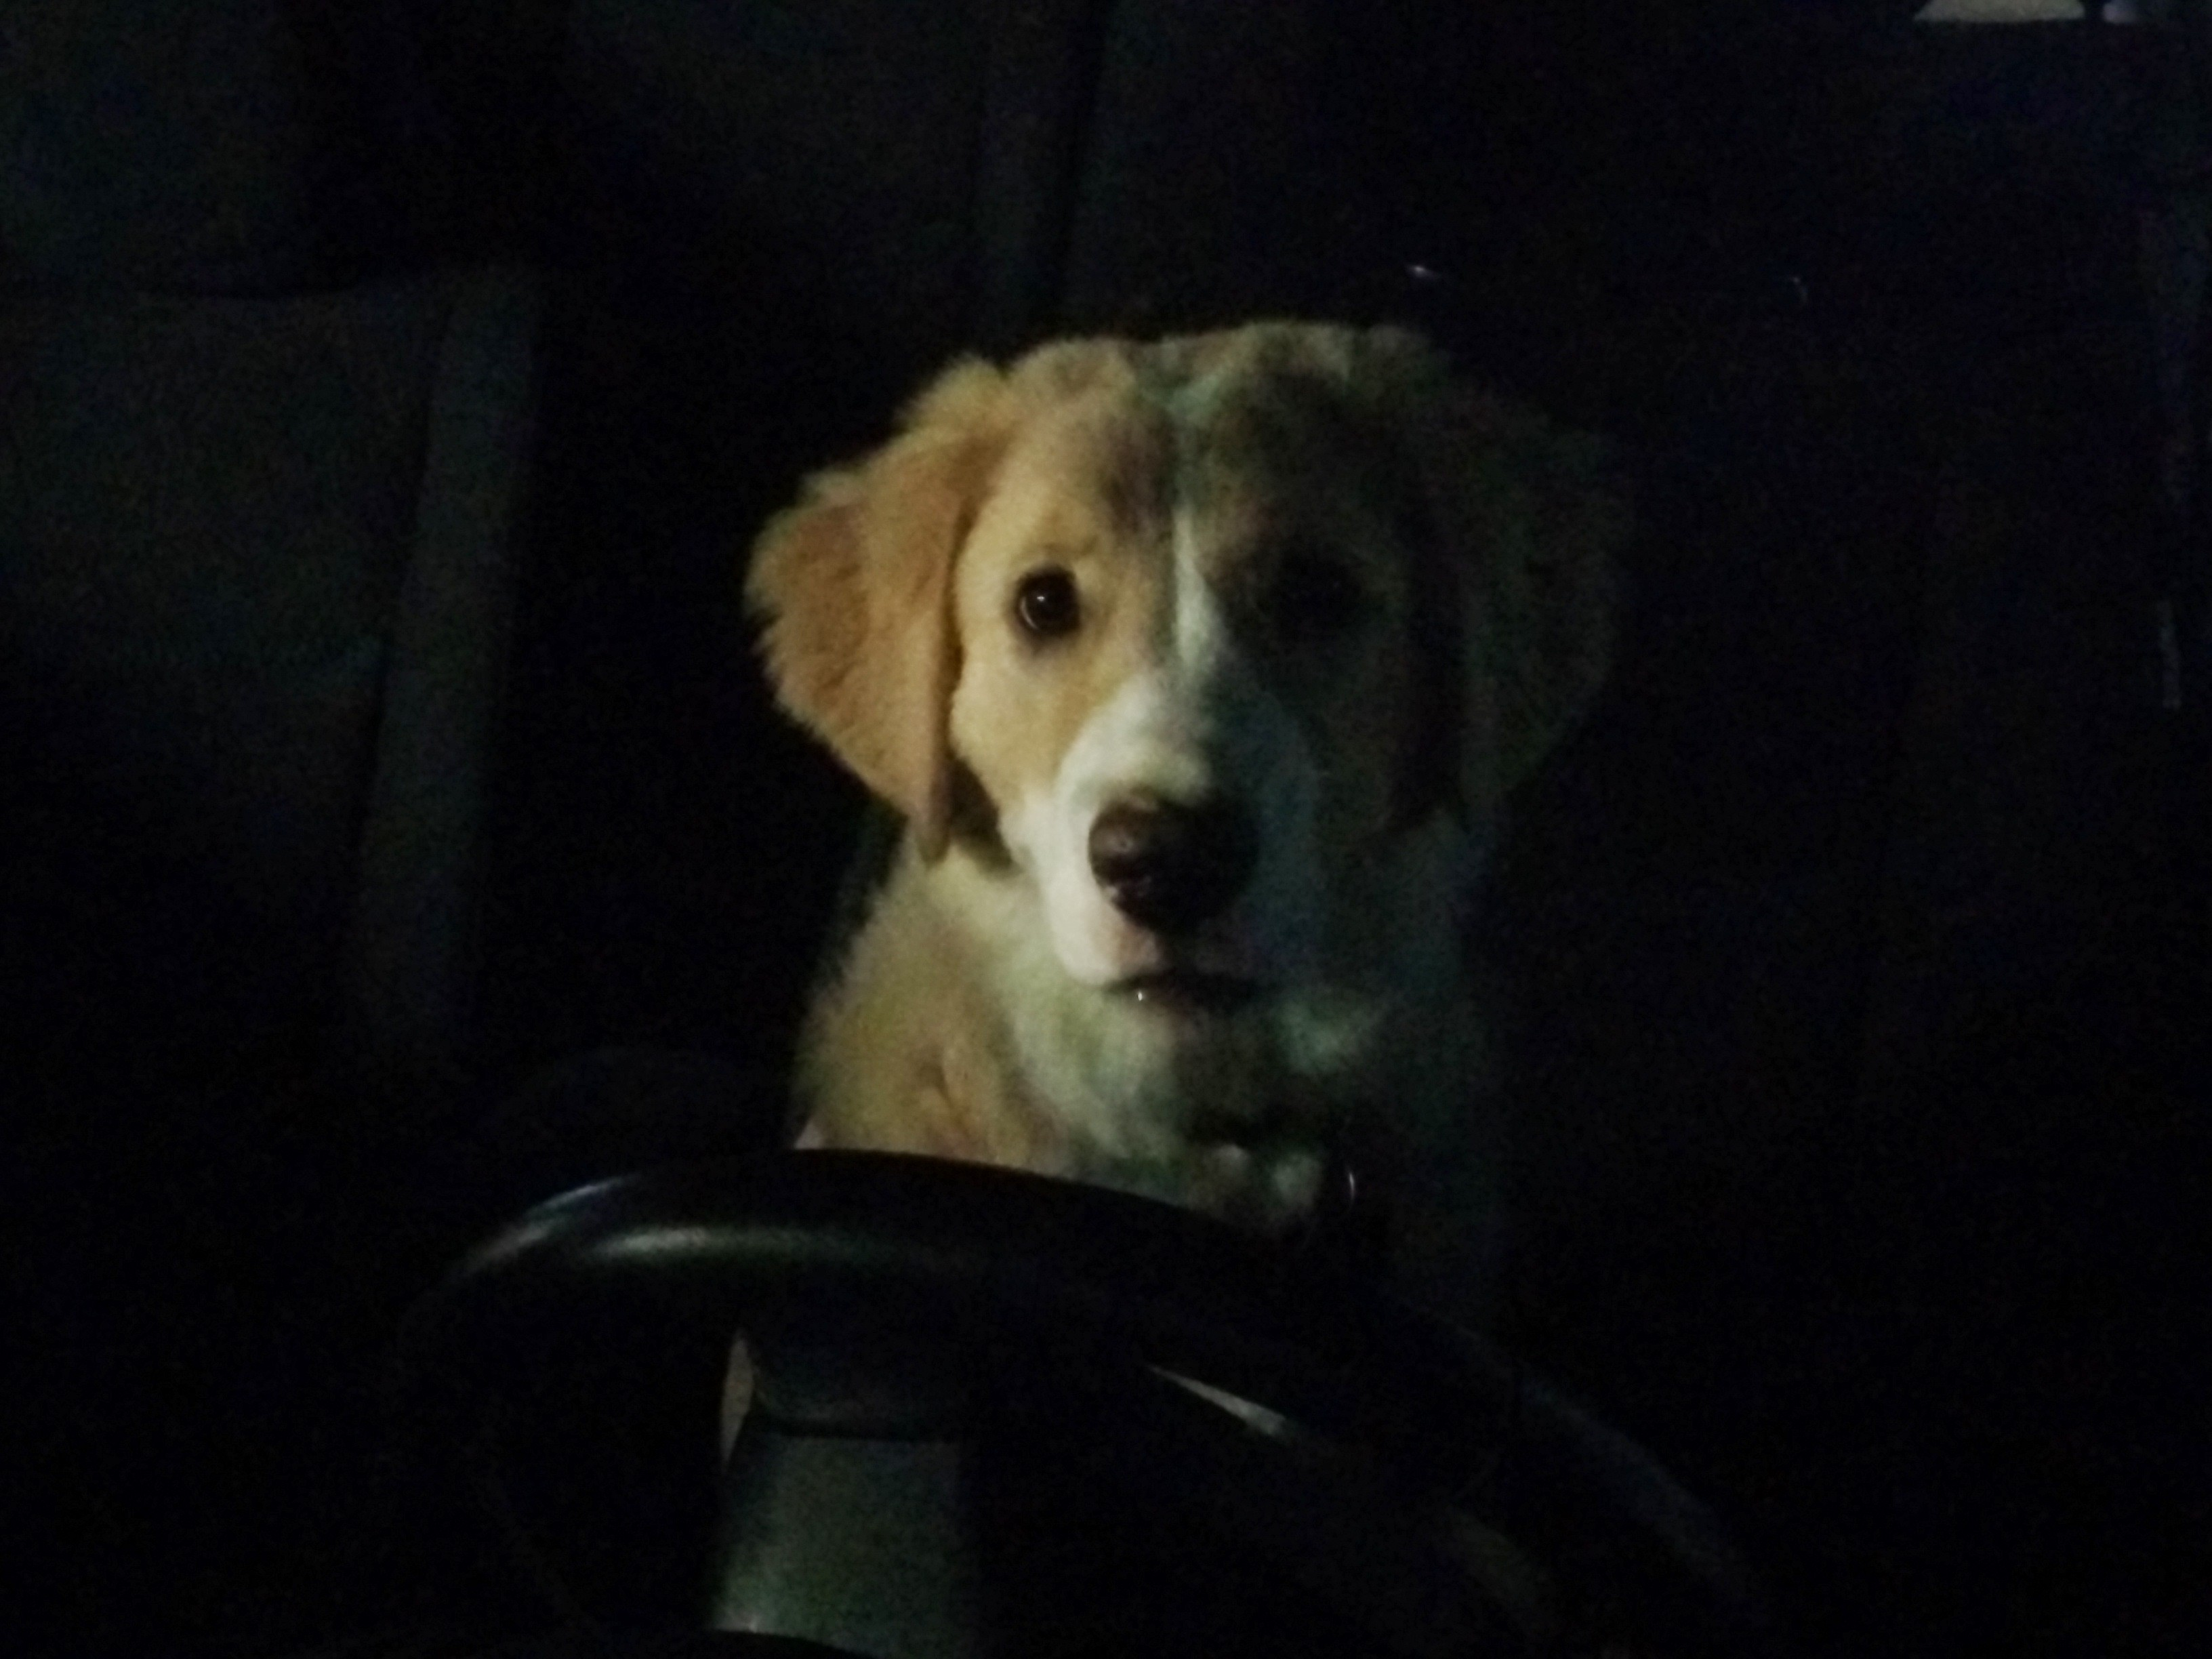
\includegraphics[width=.75\textwidth]{./images/max/title.jpg}
            \caption{Maxwell learning to operate a motor-vehicle.}
            \label{fig:max_title}
        \end{figure}

        % Bottom of the page
        \vfill
        {
            \large \theauthor \  --- \large \thedate
        }

    \end{center}
\end{titlepage}


% Contents
\newpage
\tableofcontents

% Figures
\newpage
\listoffigures

% Document
\newpage
\pagenumbering{arabic}

\section{Introduction}

So, you've been wrangled into babysitting a dog. Not just any dog though, Max.
\emph{Sigh.} What are you going to do? Maxwell Katz (no middle name) is a
rambunctions, destructive, incorrigible goofball, yet he will tug at your
heartstrings with his lovable face and ears. What should you do? What does he
eat? What does he do for fun? What should I do in the case of
emergency?! \emph{Oh no!} This may seem like a lot to handle, but fear not, 
all of this and more will be answered in the manual.

\bigskip

\begin{figure}[h!]
    \centering
    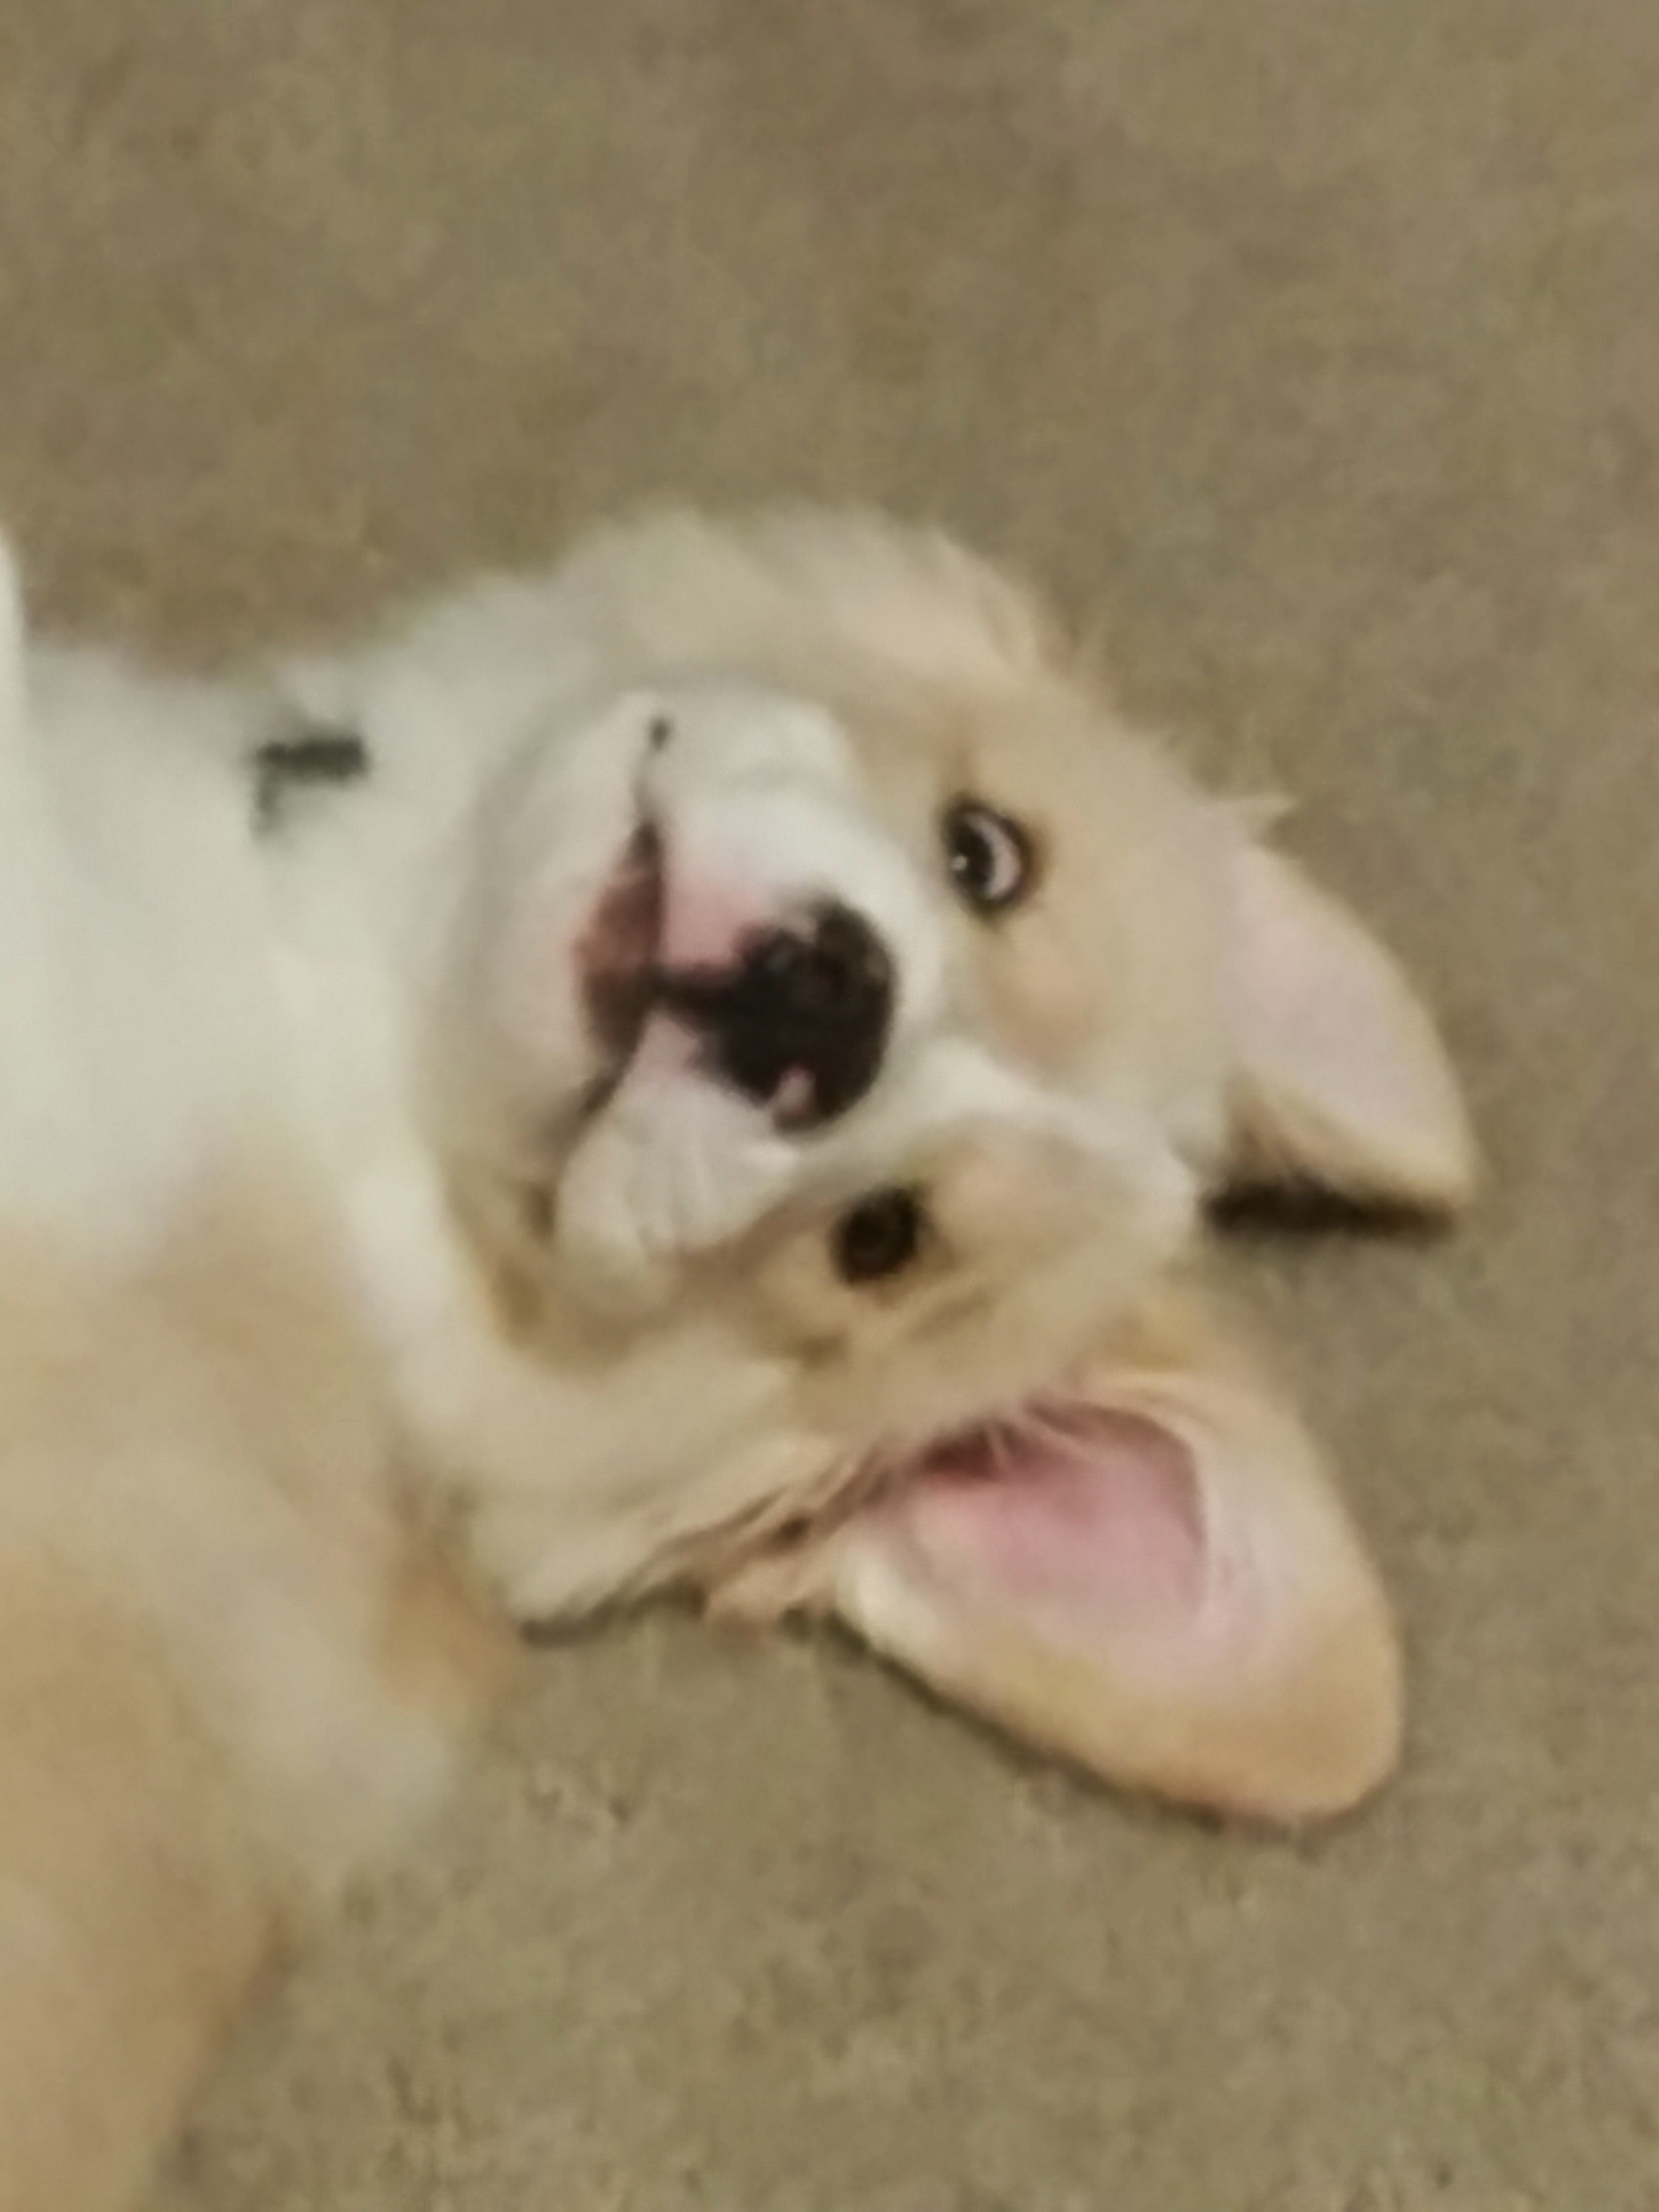
\includegraphics[width=.35\textwidth]{./images/max/crazy_eyes.jpg}
    \caption{"He's got those crazy eyes\ldots"}
    \label{fig:crazy_eyes}
\end{figure}

\newpage
\section{Emergency Information}

\begin{table}[H]
    \begin{longtable}{@{}ll@{}}
        \toprule
        \multicolumn{2}{c}{Pet Information}                                                                              \\ \midrule
        Name          & Maxwell Katz                                                                                     \\
        Answers to    & "Max!" "Maxwell" "*whistle* Come here!"                                                          \\
        Breed         & Golden Retriever / Great Pyrenees                                                                \\
        Color         & Golden White (Toasted Marsh-mellow)                                                              \\
        Weight        & 55 lbs                                                                                           \\
        Date of Birth & January 9th, 2014                                                                                \\
        Health Issues & N/A                                                                                              \\
        Allergies     & Chocolate                                                                                        \\
        Other         & Has 2 extra toes, a trait of Pyrenees                                                            \\ \midrule
        \multicolumn{2}{c}{Owner Information}                                                                            \\ \midrule
        Name          & Harrison John Katz                                                                               \\
        Phone \#      & 706.801.5289                                                                                     \\
        Email         & hjkatz03@gmail.com                                                                               \\ \midrule
        \multicolumn{2}{c}{Emergency Contact}                                                                            \\ \midrule
        Name          & Laura Katz                                                                                       \\
        Relation      & Mother of Harrison Katz                                                                          \\
        Phone \#      & 706.612.4572                                                                                     \\
        Email         & ldkatz38@gmail.com                                                                               \\ \midrule
        \multicolumn{2}{c}{Veterinary Information}                                                                       \\ \midrule
        Name          & Peachtree Hills Animal Hospital                                                                  \\
        Phone \#      & 404.812.9880                                                                                     \\
        Address       & \multirow{3}{*}{\begin{tabular}[c]{@{}l@{}}3106 Early Street\\ Atlanta, GA\\ 30305\end{tabular}} \\
                      &                                                                                                  \\
                      &                                                                                                  \\
        Website       & \url{http://www.peachtreehillsvet.com}                                                           \\
        Email         & info@peachtreehillsvet.com                                                                       \\
        Hours         & Monday-Friday, 8am-6pm                                                                           \\
        Emergency     & \url{http://www.peachtreehillsvet.com/emergencies}                                            
    \end{longtable}
    \label{tab:information}
\end{table}

\newpage
\section{Schedule}

Maxwell's schedule is extremely rigourous, and must be kept with the up most
scrutiny. He requires attention literally 24 hours a day, 7 days a week, and
without this given to him, I fear he may become deprived, depressed, or
worse\ldots dead. Below is his main schedule for a normal week, keep in mind that
Maxwell is crate trained. His crate is a safe zone, a home away from home. Feel
free to place Max in his crate whenever he becomes too much of a hazard.

\subsection{Weekly Schedule}

\begin{table}[h]
    \caption{Maxwell's rigorous daily schedule.}
    \begin{longtable}{r|ll}
                        & Weekday               & Weekend               \\ \hline \\
        Midnight - 7 am & Sleeping
                          \tablefootnote{See Fig~\ref{fig:sleeping} on
                              page~\pageref{fig:sleeping}}
                                                & Sleeping              \\
        8 am            & Morning Walk (E,O)
                          \tablefootnote{Pee and Poop}
                                                & Morning Walk (E,O)    \\
        9 am            & Breakfast             & Breakfast             \\
        10 am           & Sleeping              & Play Time             \\
        11 am           & Sleeping              & Play Time             \\
        Noon            & Sleeping              & Afternoon Walk (E)
                                                  \tablefootnote{Pee only}
                                                                        \\
        1 pm            & Sleeping              & Play Time             \\
        2 pm            & Sleeping              & Park Time             \\
        3 pm            & Sleeping              & Nap Time              \\
        4 pm            & Sleeping              & Nap Time              \\
        5 pm            & Evening Walk (E)      & Evening Walk (E)      \\
        6 pm            & Dinner                & Dinner                \\
        7 pm            & After Dinner Walk (O)
                          \tablefootnote{Poop only}
                                                & After Dinner Walk (O) \\
        8 pm            & Play Time             & Play Time             \\
        9 pm            & Play Time             & Play Time             \\
        10 pm           & Night Walk (E)        & Night Walk (E)        \\
        11 pm           & Sleeping              & Sleeping              \\
    \end{longtable}
    \label{tab:schedule}
\end{table}

\pagebreak

\subsection{Schedule Description}

As you should be able to tell by now, this is a sarcastic document. I hope that
you read the whole file, although all the basic information will be presented in
tables and lists. Below you will find a descriptive list of Max's rituals.

\bigskip

\begin{itemize}\label{itm:schedule}
    \item \textbf{Sleeping:} Max's sleeping schedule is pretty lax. He sleeps 
        quite often, and is adorable the entire time. Keep in mind the following:
        \begin{itemize}
            \item Crating Max for sleep time is OK
            \item Max can be petted while he is asleep
            \item Max sheds, so be aware of letting him on the bed
            \item Max sleeps in peculiar ways, this is OK
                  (See Fig~\ref{fig:sleeping} on page~\pageref{fig:sleeping})
        \end{itemize}
    \item \textbf{Walks:} Walking Max is a fun adventure. He is learning that he
        is strong, and WILL PULL. He has a special leash that can be used if he 
        gets out of hand. See how to put on the Easy Walk Harness on
        page~\pageref{itm:how_to_harness}.
        \begin{itemize}
            \item Walks can be as short as 30 secs, or as long as 30 mins
            \item Some walks are pee, some poop, some both
                  (See Table~\ref{tab:schedule} on page~\pageref{tab:schedule})
            \item Maxwell is trained to go to the bathroom on command
                  (See Table~\ref{tab:commands} on page~\pageref{tab:commands})
            \item Always walk Max on a leash
        \end{itemize}
    \item \textbf{Feeding:} Maxwell eats twice a day, once in the morning and
        once in the evening. He also receives water during each meal.
        \begin{itemize}
            \item Each meal consists of 1.5 cups of dog food
                  (See Fig~\ref{fig:food_bowl_filled} on
                  page~\pageref{fig:food_bowl_filled})
            \item Max is trained to wait til eating
                  (See Fig~\ref{fig:food_container_open} on
                  page~\pageref{fig:food_container_open})
            \item Max eats fast, and he must be walked immediatly after dinner
        \end{itemize}
    \item \textbf{Play Time:} Max loves to play! He plays ball, tug of war, chew
        the shoes, eat the garbage, and lots more\ldots!
        \begin{itemize}
            \item Max comes with a plethera of toys
                  (See List~\ref{itm:included_items} on
                  page~\pageref{itm:included_items})
            \item Max loves to play in the dirt and mud
            \item Max is very energetic, you have been warned
                  (See Fig~\ref{fig:at_the_park} on
                  page~\pageref{fig:at_the_park})
        \end{itemize}
\end{itemize}

\bigskip

\begin{figure}[h!]
    \centering
    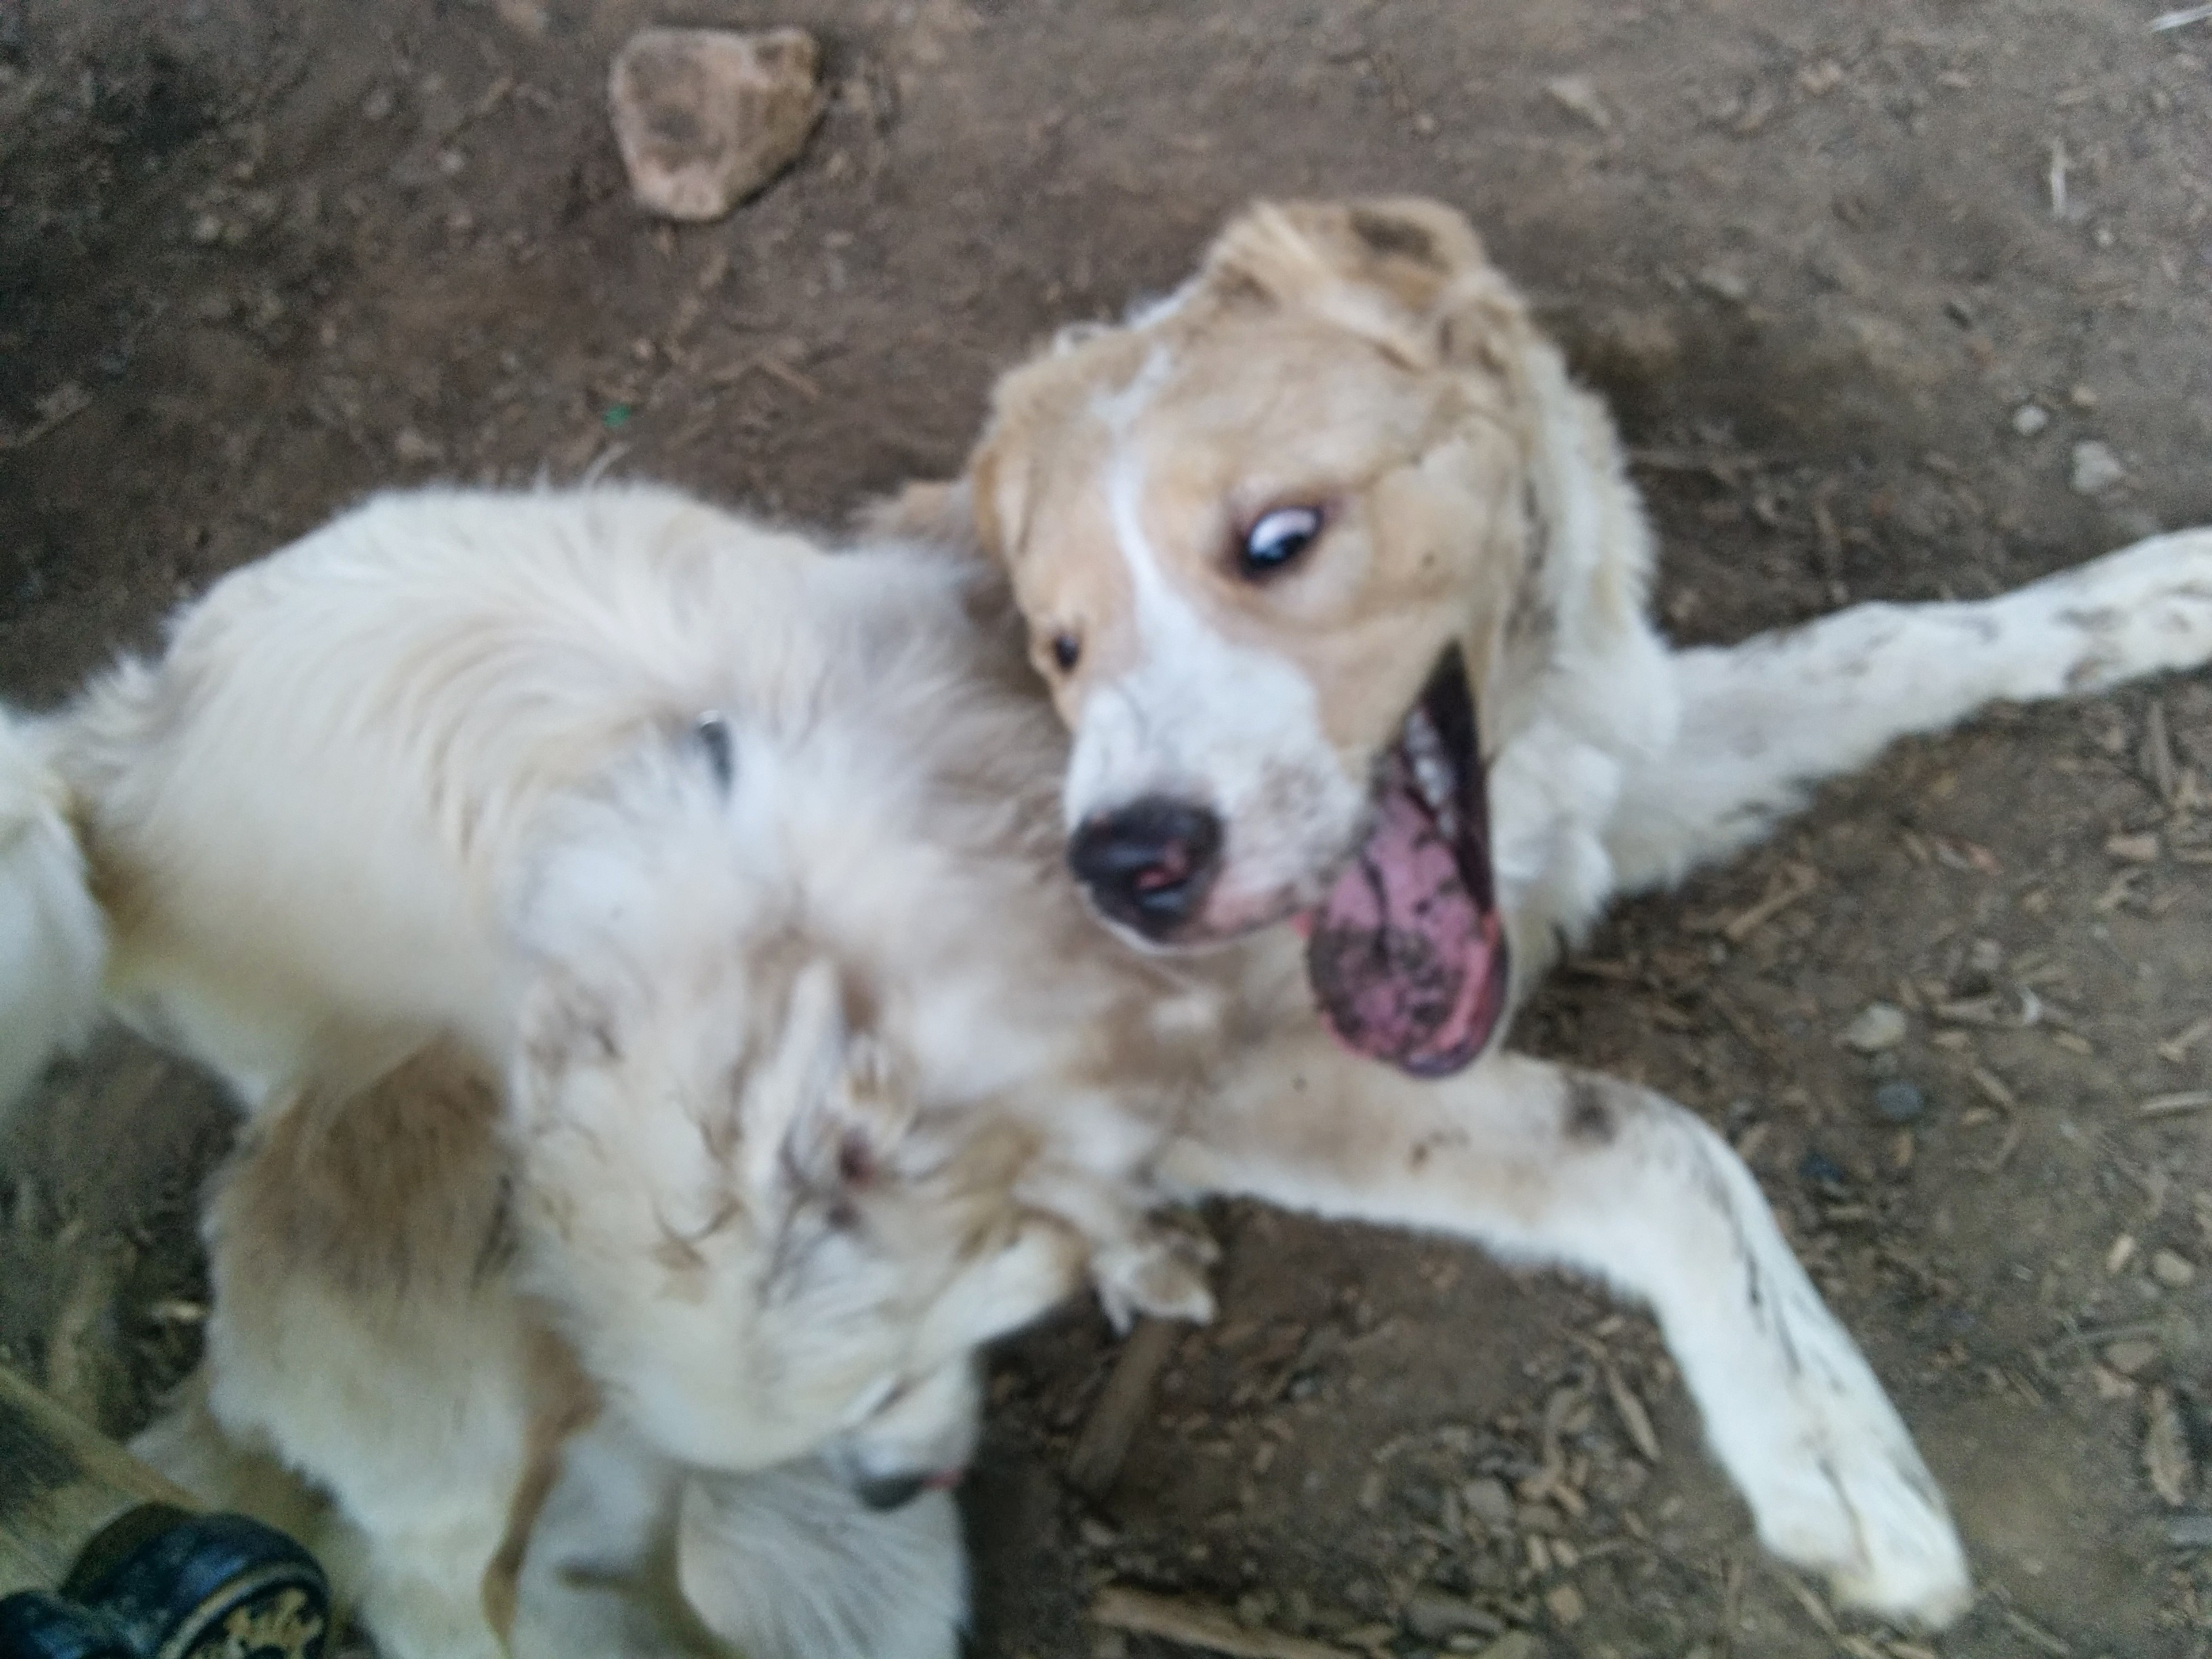
\includegraphics[width=.35\textwidth]{./images/max/at_the_park.jpg}
    \caption{Maxwell playing at the park.}
    \label{fig:at_the_park}
\end{figure}

\bigskip

\begin{figure}[h!]
    \centering
    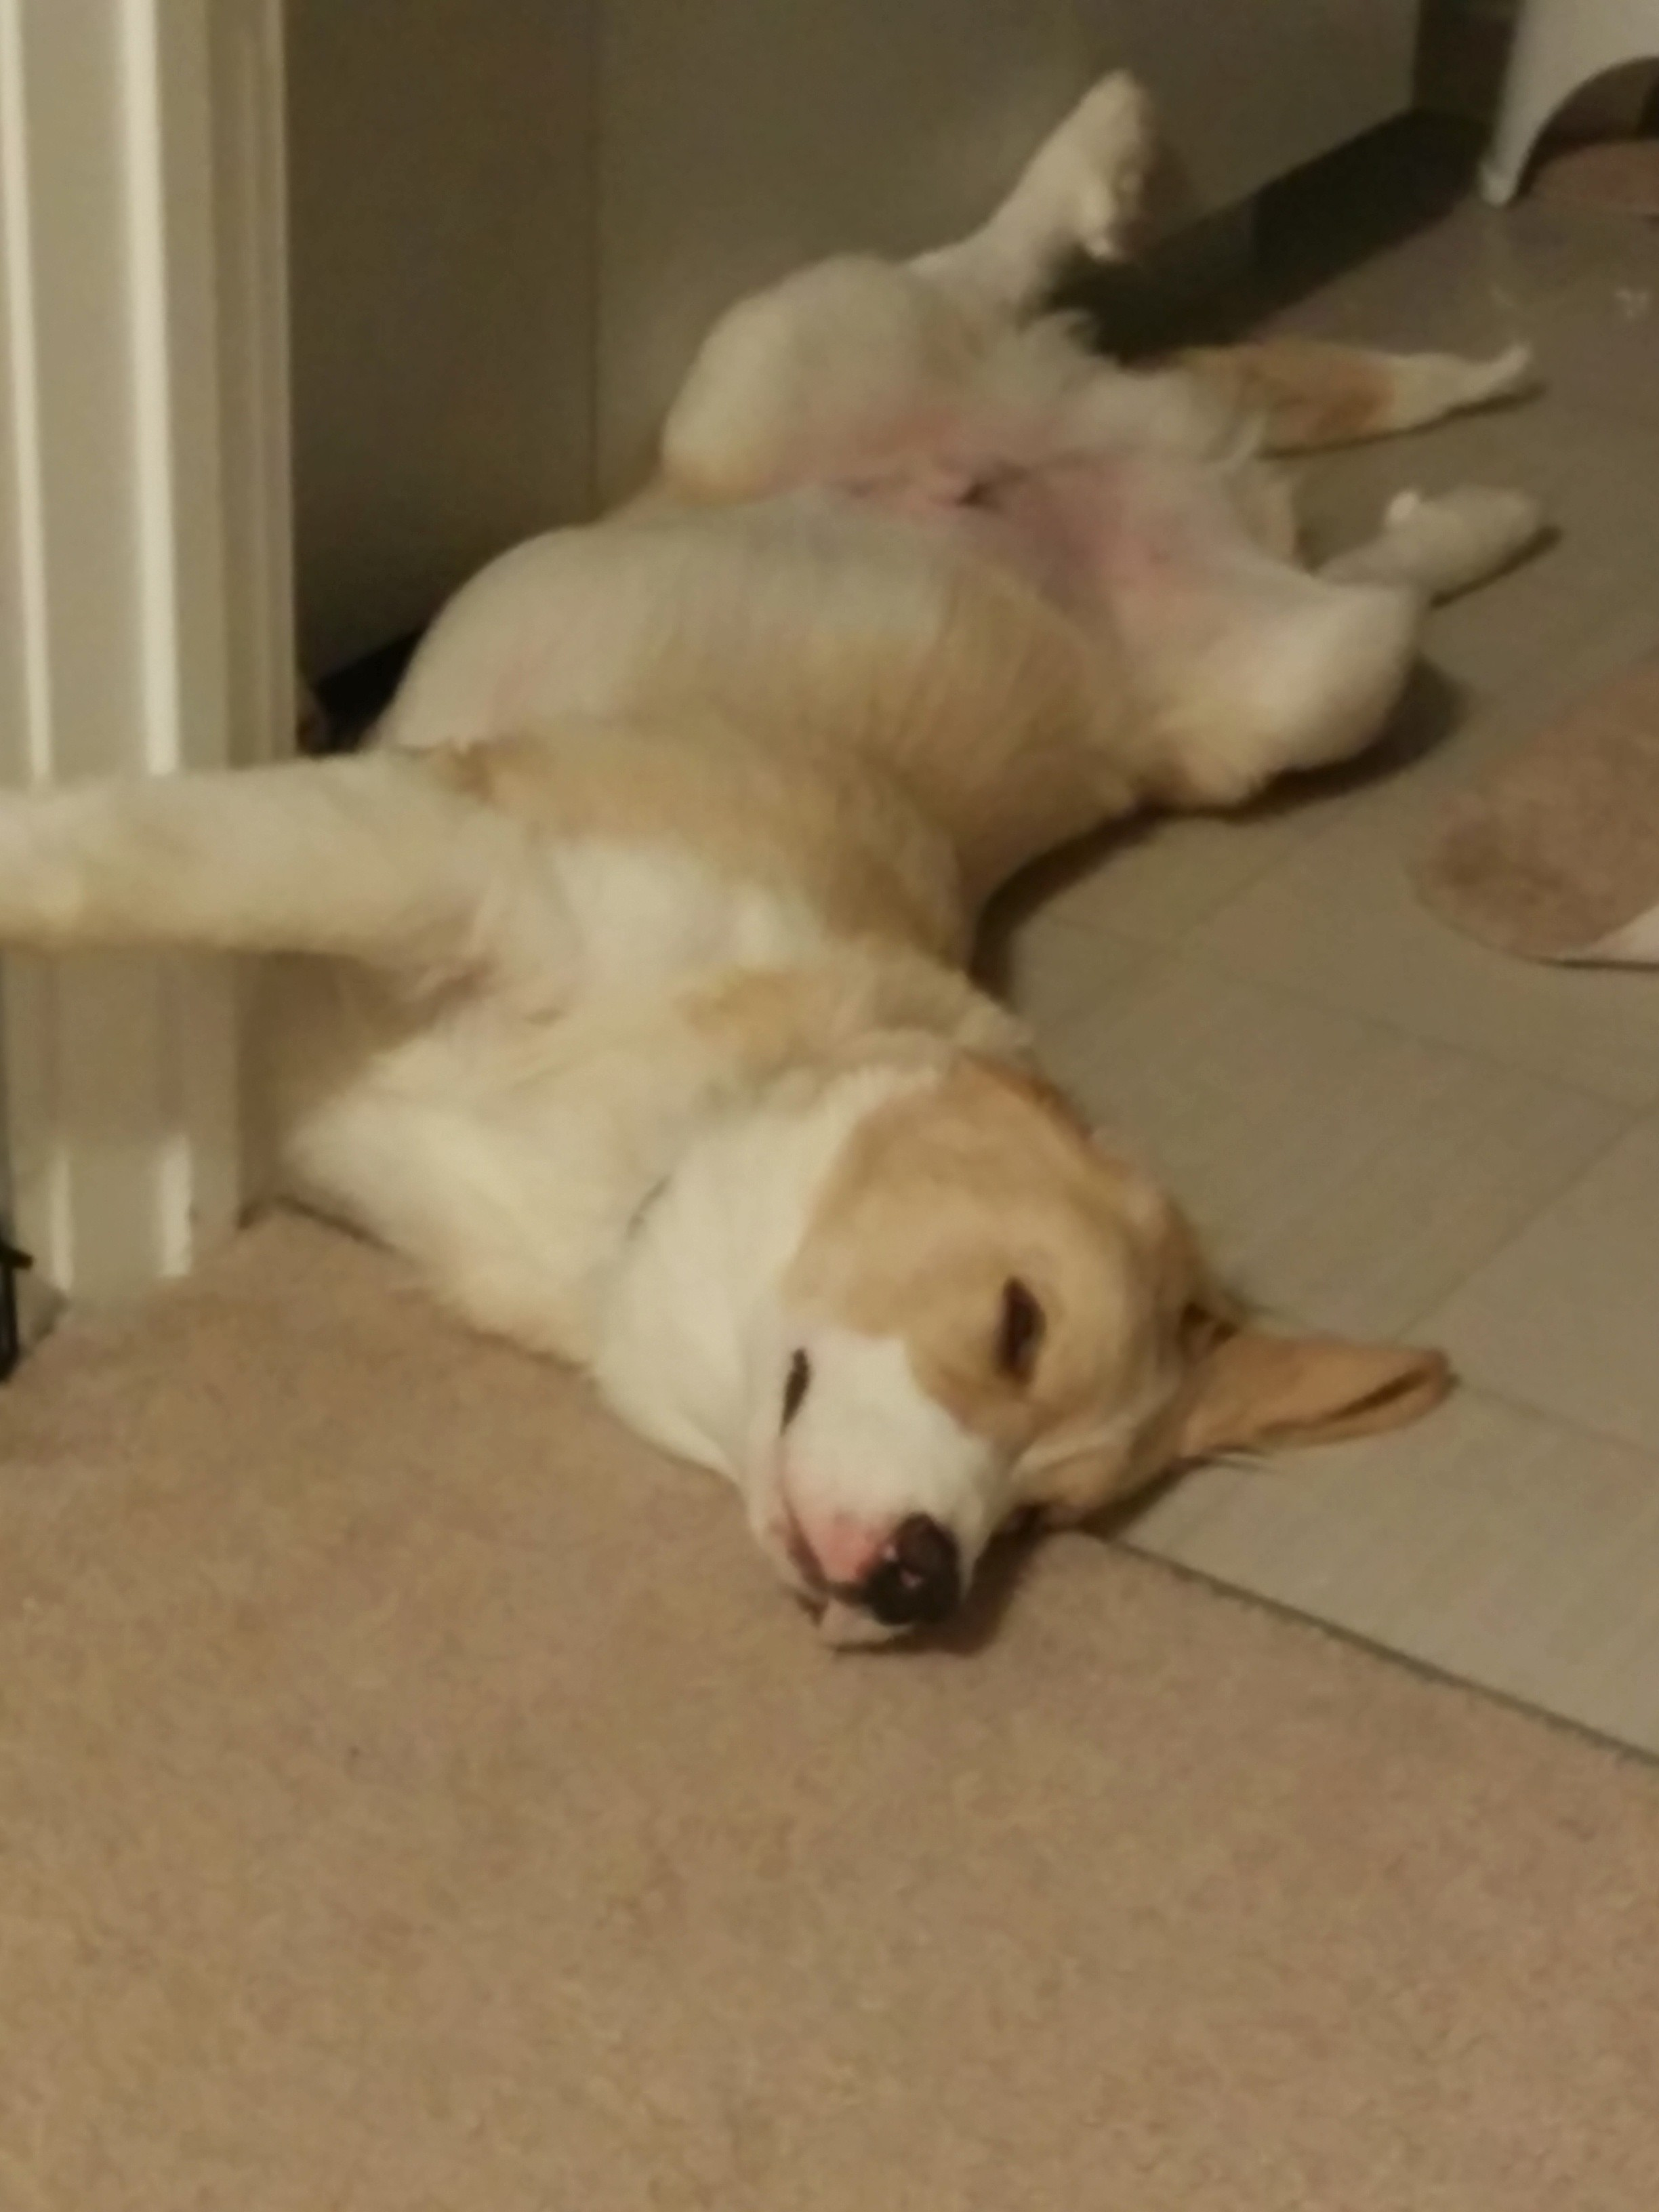
\includegraphics[width=.35\textwidth]{./images/max/sleeping.jpg}
    \caption{Maxwell sleeping normally\ldots mostly\ldots}
    \label{fig:sleeping}
\end{figure}

\bigskip

\clearpage
\newpage
\section{Included Items}

Here is a list of all of the items that you will receive for watching Maxwell.
Most of it will be in his bag. You will not need to use all of these items, and
don't worry if things get lost. In all honesty Max will probably find a toy to
take home, and one to leave there. You have been warned.

\begin{enumerate}\label{itm:included_items}
    \item Maxwell Katz
    \item Crate Items
        \begin{enumerate}
            \item Metal Frame
            \item Plastic Base
            \item Max's Towel
        \end{enumerate}
    \item Max's Bag
        \begin{enumerate}
            \item Carrying Bag
            \item Treats
            \item Kong Filling
            \item Nail Clippers
            \item Bitter Spray
            \item Baggies
            \item Peepee Spray
            \item Good Paper Towels
            \item Furminator Brush
            \item Shampoo
            \item Toys
                \begin{enumerate}
                    \item Elk Antler
                    \item Tennis Ball
                    \item Tug of War
                    \item Kong Ball
                    \item Chew Treats
                \end{enumerate}
        \end{enumerate}
    \item Food Bowls (x2)
    \item Feeding Container
    \item Leash
\end{enumerate}

\newpage
\section{Commands}

This section is all about how to speak to Max. You need to be commanding yet
attentive to his mood. Like all animals, he demands respect, and misbehaves like
a child would. He will always listen to commands better with a treat/toy in
hand. Maxwell has also been trained to listen for whistling, any command can be
prefaced with a short loop-de-loop whistle to make him pay attention.

\begin{table}[H]
\label{tab:commands}
\begin{adjustwidth}{-4.5cm}{-4.5cm}
\begin{center}
    \begin{tabular}{lp{.3\textwidth}p{.3\textwidth}p{.3\textwidth}}
        Command     & Hand Motion                                      &
        Description                                           & Notes
        \\ \hline \\
        Bad Dog     & N/A                                              & Term of extreme discipline                            & Shouted with angry eyes                                            \\
        Come Here   & *snap* Point to side                             & Get Maxwell to come to you                            & Should be prefaced with Maxwell                                    \\
        Down        & Pinched fingers, downward bow motion             & Laying down                                           & Sit, then down                                                     \\
        Drop it     & Hold hand below mouth for item                   & Drops item in mouth / opens mouth                     & Need to "trade" another item for what he has                       \\
        Eh! / Uh-uh & N/A                                              & General purpose use, stop what Max is currently doing &                                                                    \\
        Fetch       & Throwing motion                                  & Go get
        what I threw for you\ldots dummy                   &                                                                    \\
        Go          & Herding motion with both hands                   & Move out of my way, go somewhere                      & Use for getting him into his crate                                 \\
        Good Boy    & Petting, Smiling                                 & Term of praise                                        &                                                                    \\
        Go Outside  & N/A                                              & Get Maxwell excited, go to the door                   & Ask as a question                    \\
        Leave it    & Yank leash                                       & Leave it alone, ignore it                             & Start with Eh / Uh-uh                                              \\
        Maxwell     & N/A                                              & Get his attention                                     &                                                                    \\
        No          & N/A                                              & More extreme Eh / Uh-uh                               &                                                                    \\
        Okay        & N/A                                              & Release
        command                                       & Use to release from
        wait, sit, down, feeding, etc\ldots                \\
        Poopy       & N/A                                              & Go poop                               & For use outside                                                    \\
        Potty       & N/A                                              & Go pee                                & For use outside                                                    \\
        Sit         & Pinched fingers, upward motion                   & Sitting                                               &                                                                    \\
        Stop        & N/A                                              & Stop walking, wait for me, sit                        & Shouted, use while on leash, stop moving                           \\
        Take it     & Hand with item near mouth                        & Take this, eat this, it's okay                        &                                                                    \\
        Wait        & Hand stop signal towards his nose                & Wait here, stay                                       & Start with sit, then wait. Always release, or say Eh and try again \\
        Watch me    & Two fingers, point at Max's eyes, then your eyes & Watch me, focus                                       & "I've got my eyes on you" motion. Works well with a treat         
    \end{tabular}
\end{center}
\end{adjustwidth}
\end{table}

\newpage
\section{Rewards and Discipline}

Maxwell is still a puppy, so he is still learning. In fact he is always
learning, and like a child he is impressionable. Please keep in mind that by
accepting to watch Max that you will be expected to continue his training and
discipline.  This is not a big undertaking. 

\bigskip

Training Max is really easy and will mostly be done without a second thought.
Basically when he does something good, you praise him. And when he disobeys, you
discipline him. Praise can be in the form of treats, pets, "Good boy", and
generally loving him. Discipline can be in the form of "Eh", "No", "Bad dog",
angry eyes, and crating. 

\bigskip

Basic training to keep up with his behaivior involves sit, down, wait, come
here, and release. A basic rule of thumb is that whenever Max is going to be
rewarded, train him first. This keeps him respectful of you, and entertains him
as his breed likes to please and be challenged. When you feed him, make him sit,
then release for feeding. When you play fetch, make him sit, or down, or stay
before throwing his toy. When you enter or leave a doorway, make him sit and
wait for the door to be opened. And further training is not out of the question.
Feel free to teach him new tricks!

\bigskip

Discipline is a bit different. He will misbehave, and when he does, he must be
told. Use "Eh" and "Uh-uh" frequently. "No" and "Bad dog" should only be used
for very bad behaviours that include chewing furniture, chewing shoes, accidents
in the house, etc\ldots Below is a non-comprehensive list of what to do in
various situations.

\bigskip

\begin{enumerate}\label{itm:discipline}
    \item \textbf{Accident Indoors:} If Max has an accident inside the house,
        pleas feel free to yell! Shout "NO! Bad Dog!". Keep him from moving,
        then when he finishes, drag him by his collar to his crate. Keep him in
        timeout for approx. 20 mins.
    \item \textbf{Baring Teeth / Nipping:} If he bares his teeth or nips at you,
        firmly state "No". Then avoid eye contact.
    \item \textbf{Barking:} Firmly state "No bark." Then soothe him with a calm
        "shhhhh". If he continues, get him to sit. Then pet him and hold one
        hand under his chin while putting pressue on his vocal chords.
    \item \textbf{Biting:} If Max bites you or anyone else or anything else,
        shout "No bite!". Then kneel down and hold his mouth closed while
        maintaining eye contact. Keep a firm, yet non-squeezing grip until he
        pulls away. (Note: he might whine, this is OK)
    \item \textbf{Causing Pain:} If Maxwell truly causes you pain through a
        bite, scratch, tackle, or otherwise, shout "ouch!". This will let
        him know that he has been playing too rough, or hurt you in some way.
        Normally after this I calm him down and give him something to chew on.
    \item \textbf{Chewing:} When (not if) you catch him chewing on something hew
        shouldn't be chewing, state "No bite". Then give him a toy he can chew
        on. (See List~\ref{itm:included_items} on
        page~\pageref{itm:included_items})
    \item \textbf{Eating Something:} Again, when you catch him eating something
        he shouldn't be eating, shout "Eh". Then try the command "Drop it" (See
        Table~\ref{tab:commands} on page~\pageref{tab:commands}). If that
        doesn't work, open his mouth and remove the item.
    \item \textbf{Growling:} Calm him down with petting and a soothing "shhhh".
    \item \textbf{Playing Rough:} If Max is playing rought when he should be
        calming down, follow the above. Get him to lay down, then pet him and
        soothe him with a "shhhh".
    \item \textbf{Refusing to Listen:} Get a treat.
    \item \textbf{Refusing to Walk:} Use a firm tug with a firm "Eh".
\end{enumerate}

\bigskip

This is not an exhaustive list by any means. Generally a firm "Eh" and a stern
voice with a look of dissaproval will fix a problem temporarily. Remember that
you can always put him away in his crate as both punishment and nap time. If you
have any major problems please feel free to call, text, or email my contact
information. (See Table~\ref{tab:information} on page~\pageref{tab:information})

\newpage
\section{How to\ldots}

This section contains various instructions on how to care for Max. Each item has
a list of what you should do in this situation. Pictures are provided as a
convinence. Should you have any other questions or concerns, please contact me.
(See Table~\ref{tab:information} on page~\pageref{tab:information})

\subsection{How to feed Max}
\begin{enumerate}\label{itm:how_to_feed}
    \item Fill his water bowl $\frac{1}{2}$ way up with cold tap water
    \item Open the food container top (See Fig~\ref{fig:food_container_open})
    \item Fill his food bowl with 1.5 cups of food (See Fig~\ref{fig:food_bowl_filled})
    \item Release Max to eat
\end{enumerate}

\bigskip

\begin{figure}[h!]
    \centering
    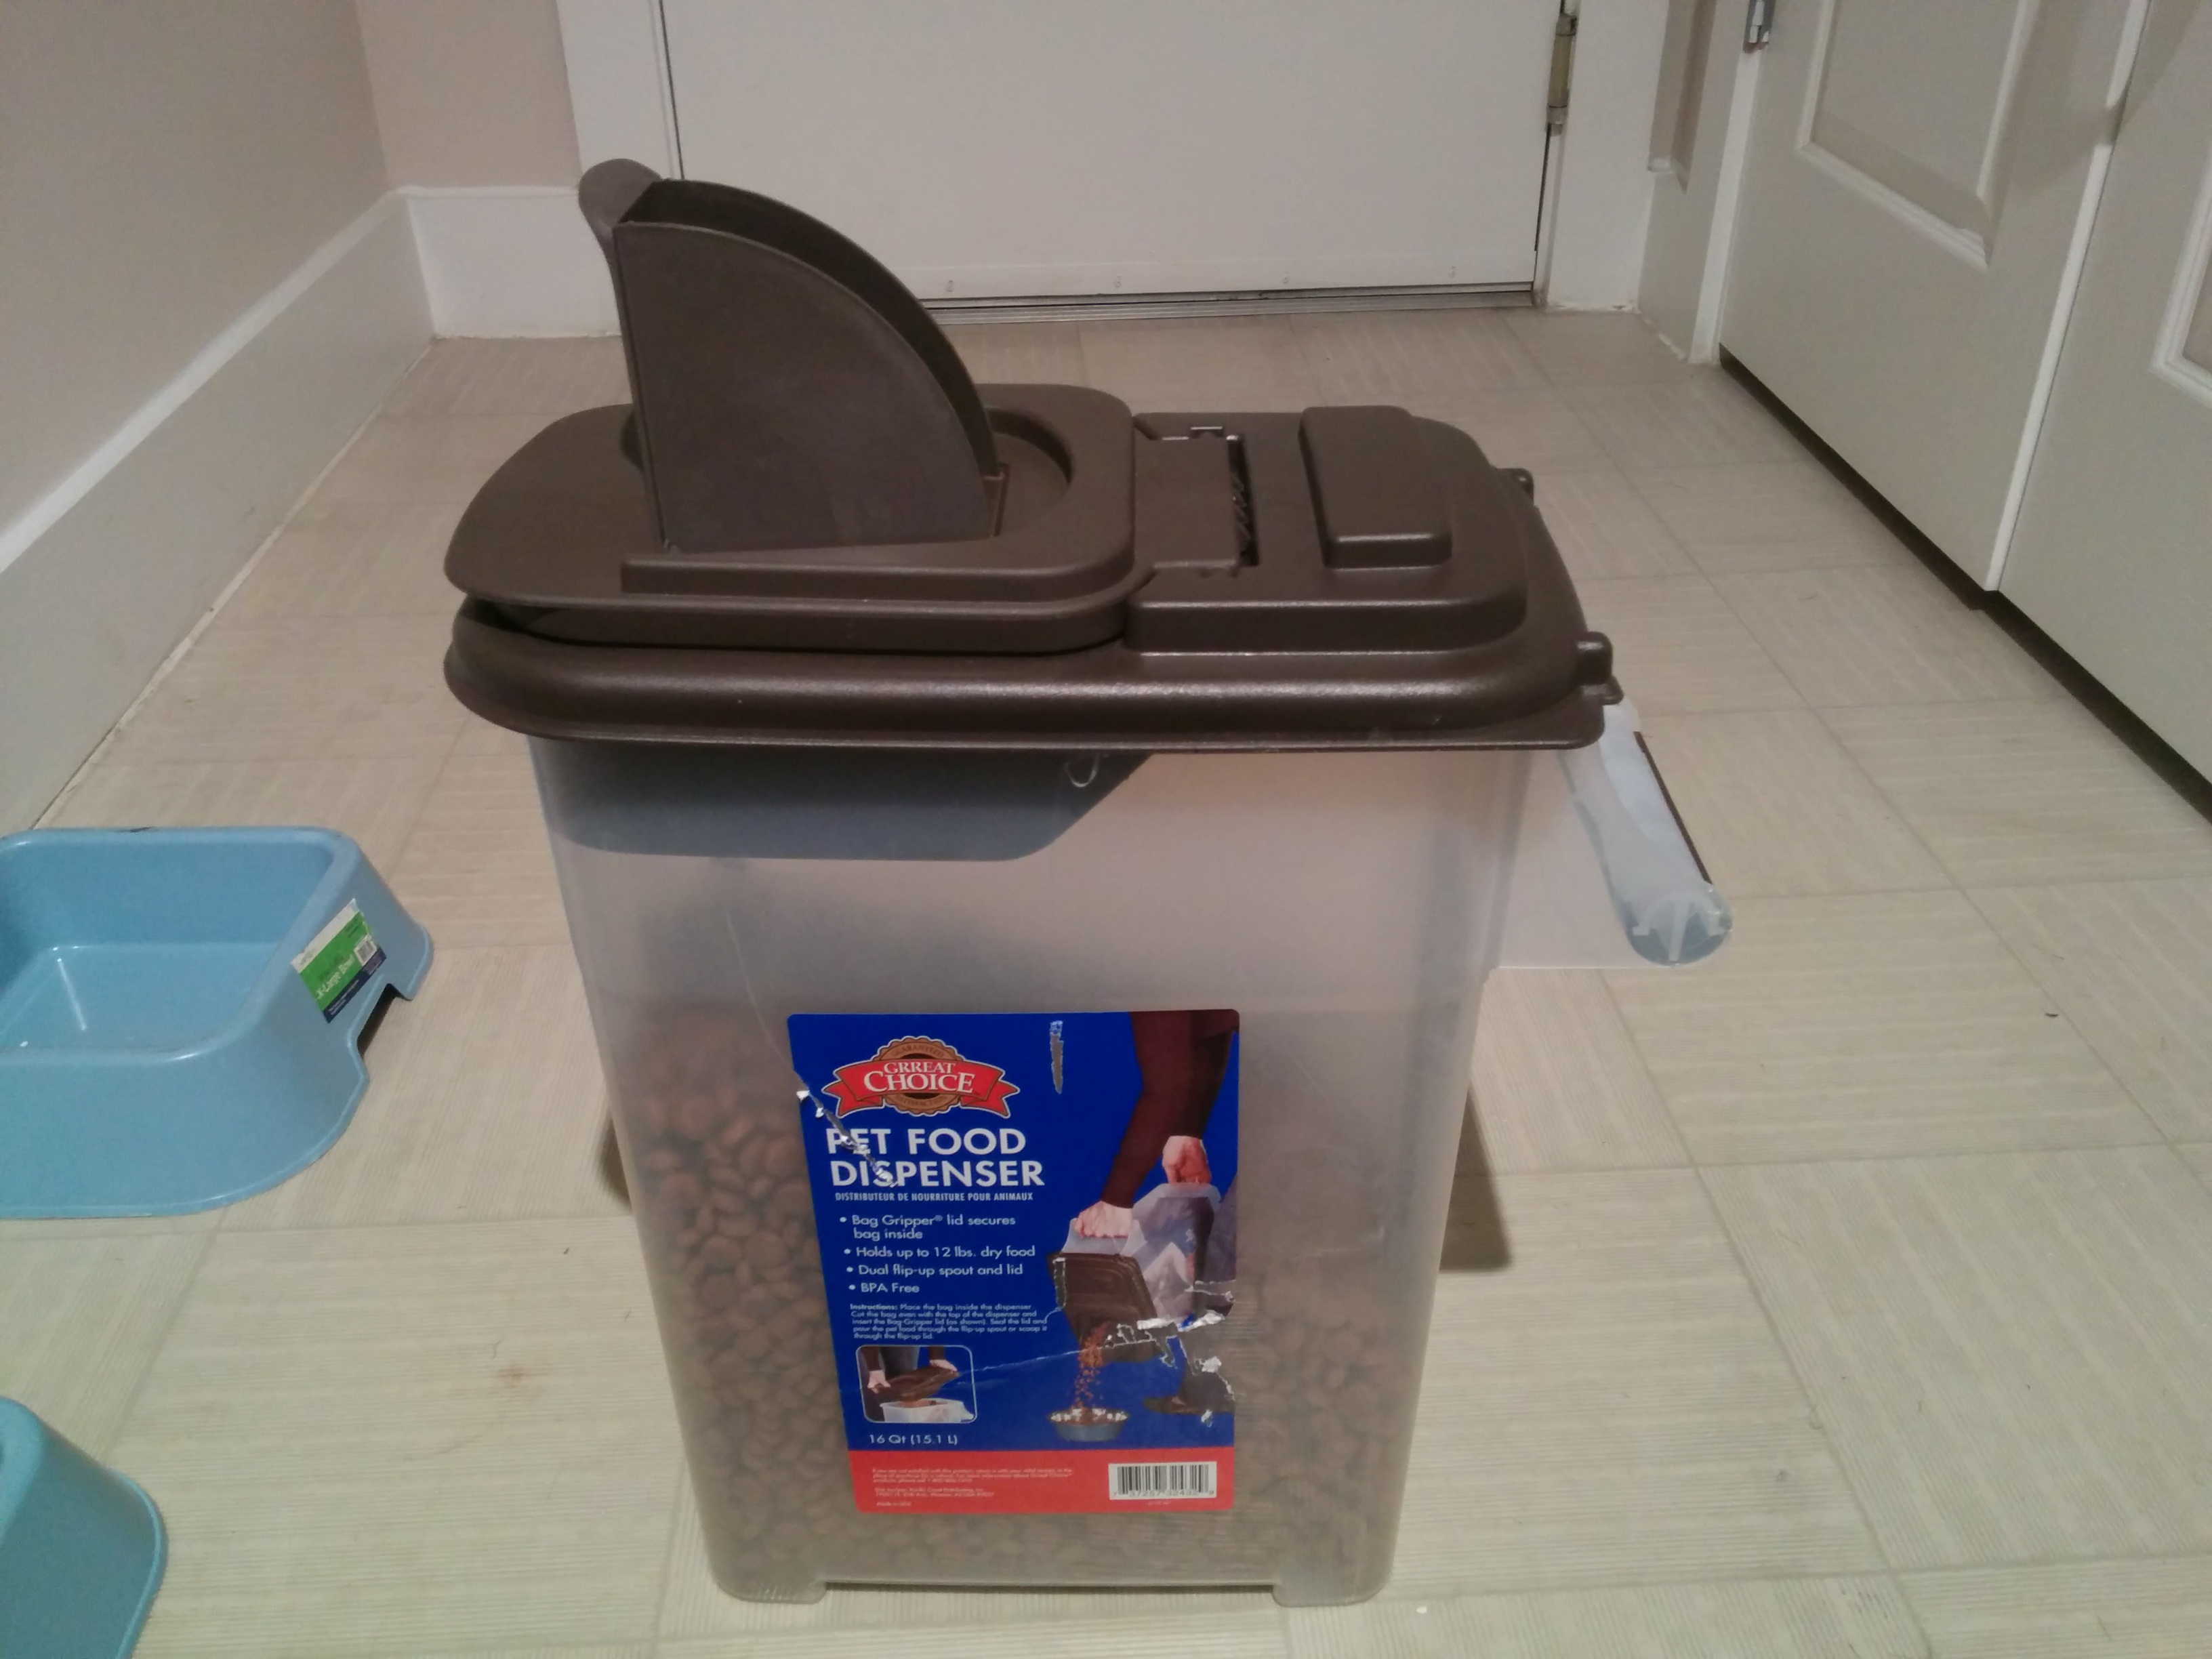
\includegraphics[width=.35\textwidth]{./images/how_to/feed_max/food_container_open.jpg}
    \caption{The food container being opened correctly.}
    \label{fig:food_container_open}
\end{figure}

\bigskip

\begin{figure}[h!]
    \centering
    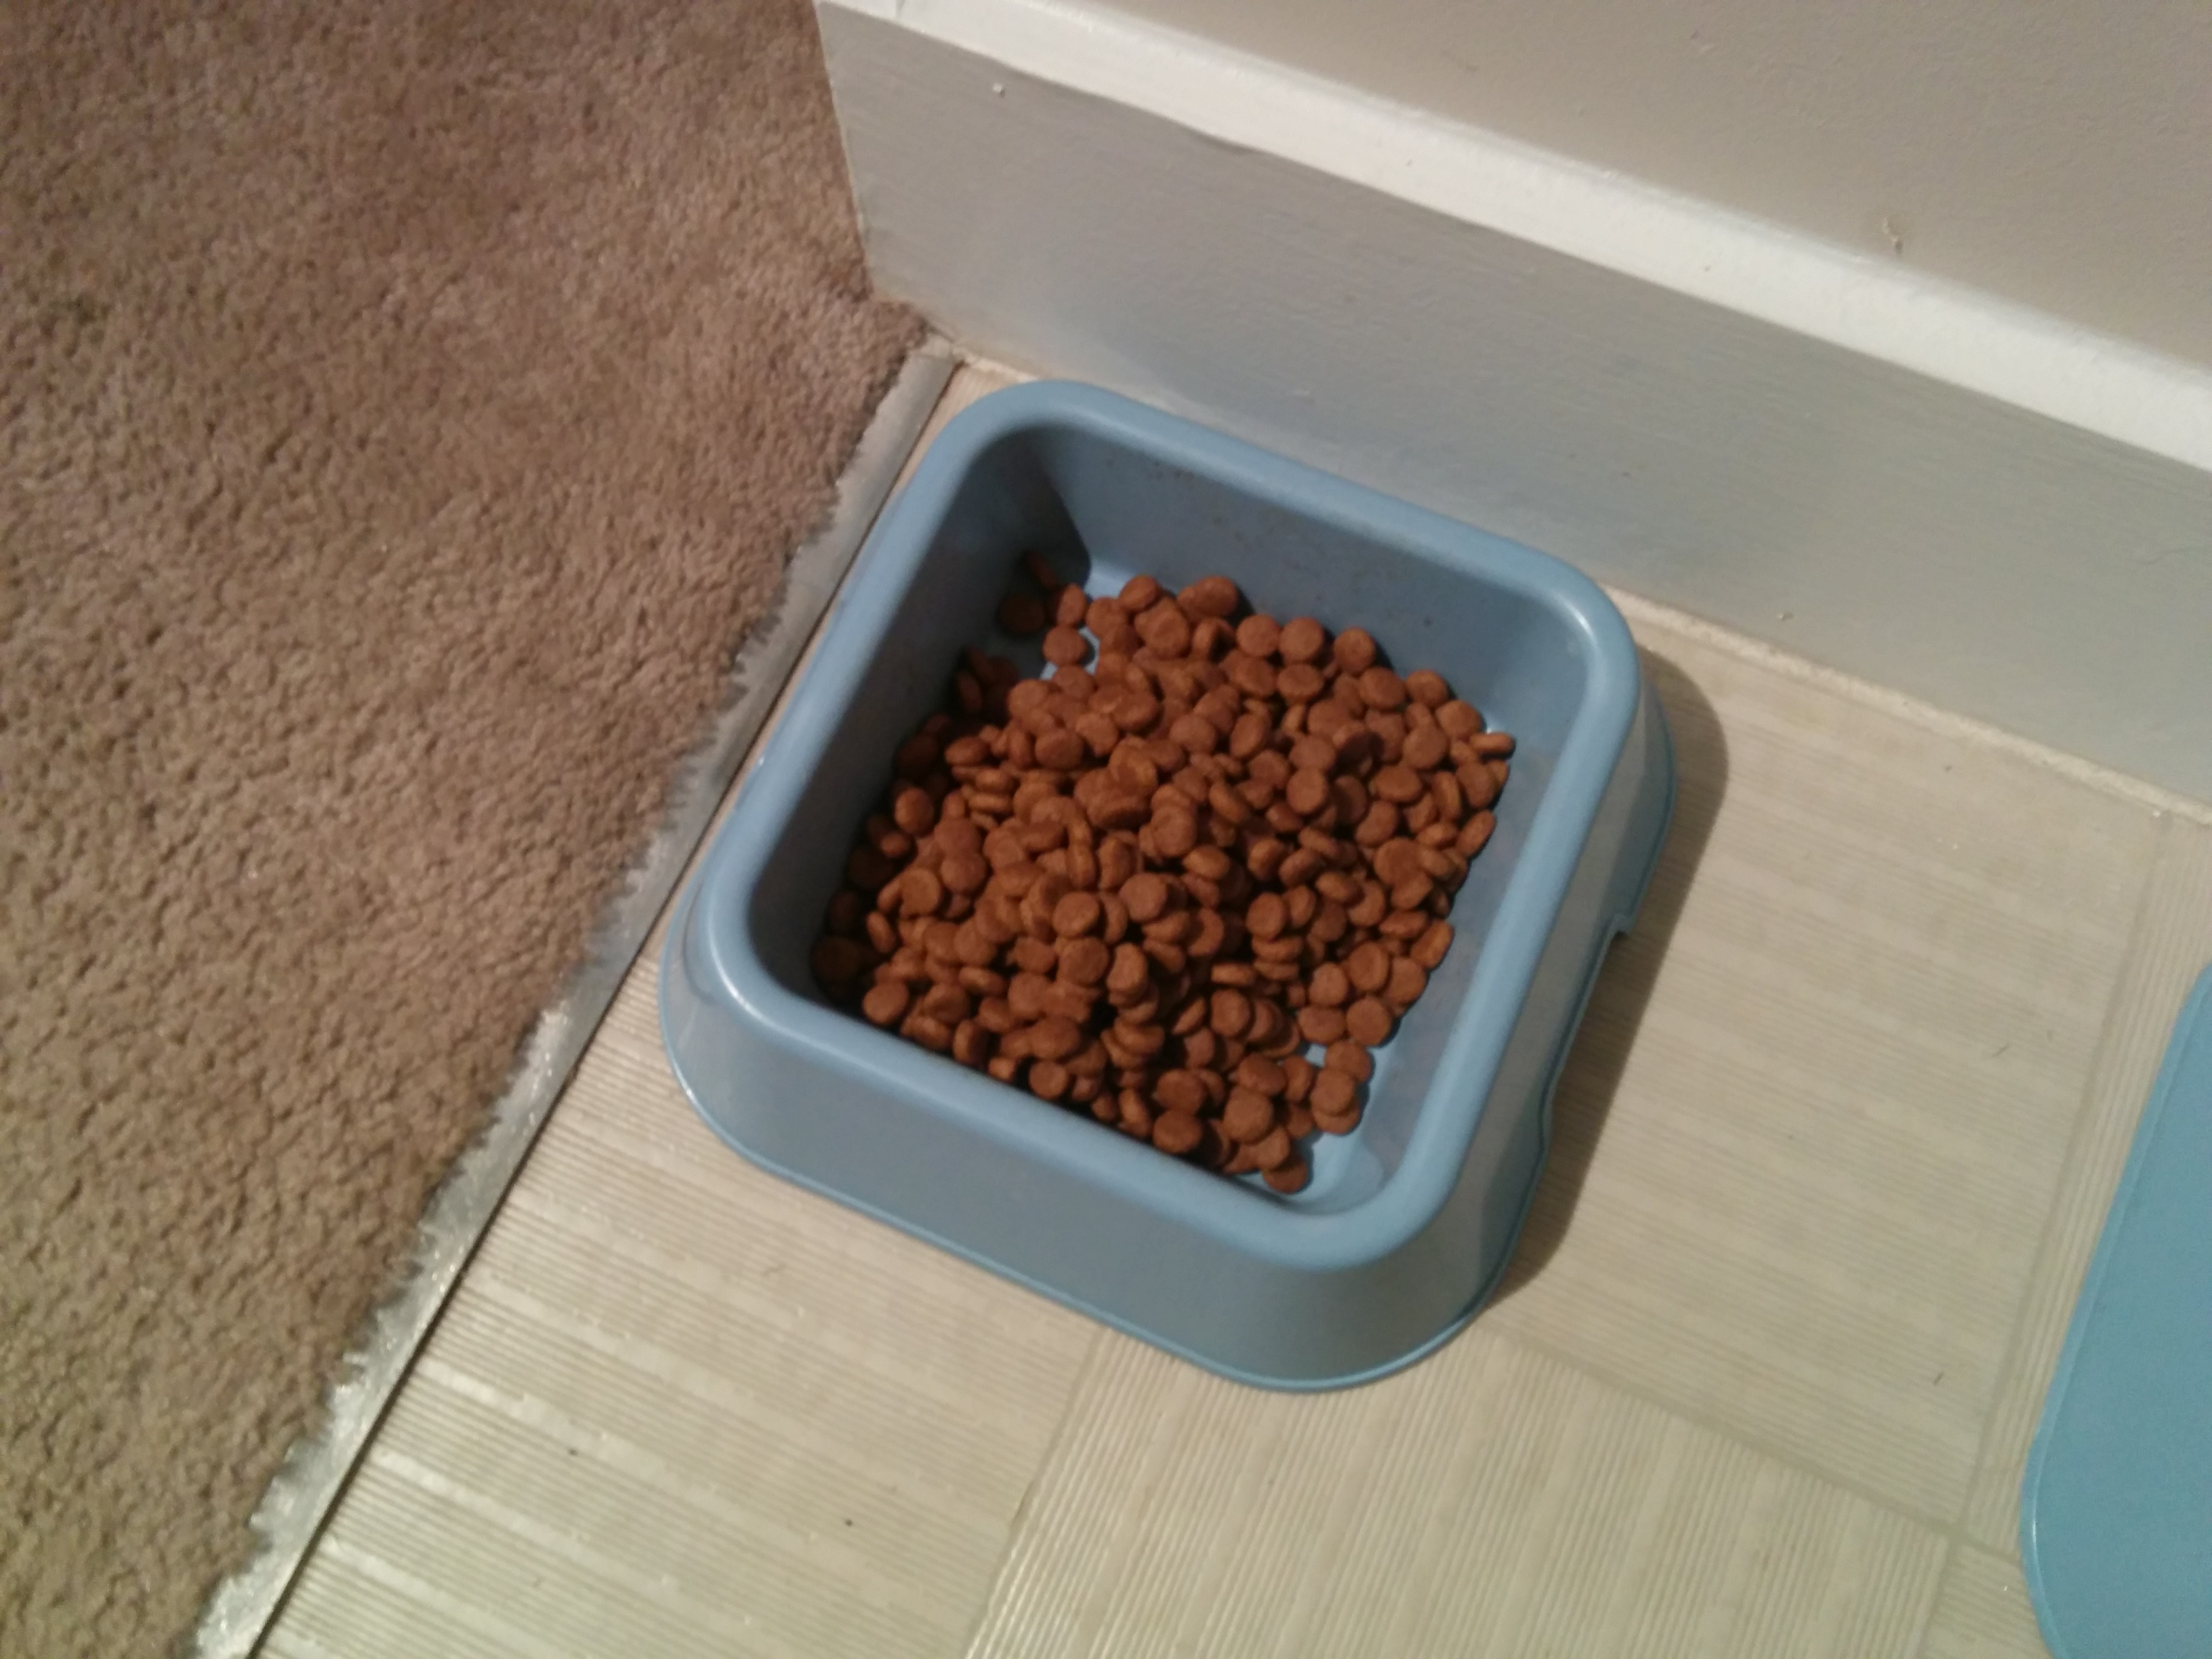
\includegraphics[width=.35\textwidth]{./images/how_to/feed_max/food_bowl_filled.jpg}
    \caption{Max's food bowl filled to the proper amount.}
    \label{fig:food_bowl_filled}
\end{figure}

\subsection{How to walk Max}
\begin{enumerate}\label{itm:how_to_walk}
    \item Call Maxwell to the door saying, "Let's go outside!"
    \item Get Maxwell to sit, waiting
    \item Put the leash on Max (either leash)
    \item Go outside, while walking keep Max on a short leash
          (See Fig~\ref{fig:walking_max})
    \item It should be loose, yet ready to tug
          (See Fig~\ref{fig:short_leash})
\end{enumerate}

\begin{figure}[H]
    \centering
    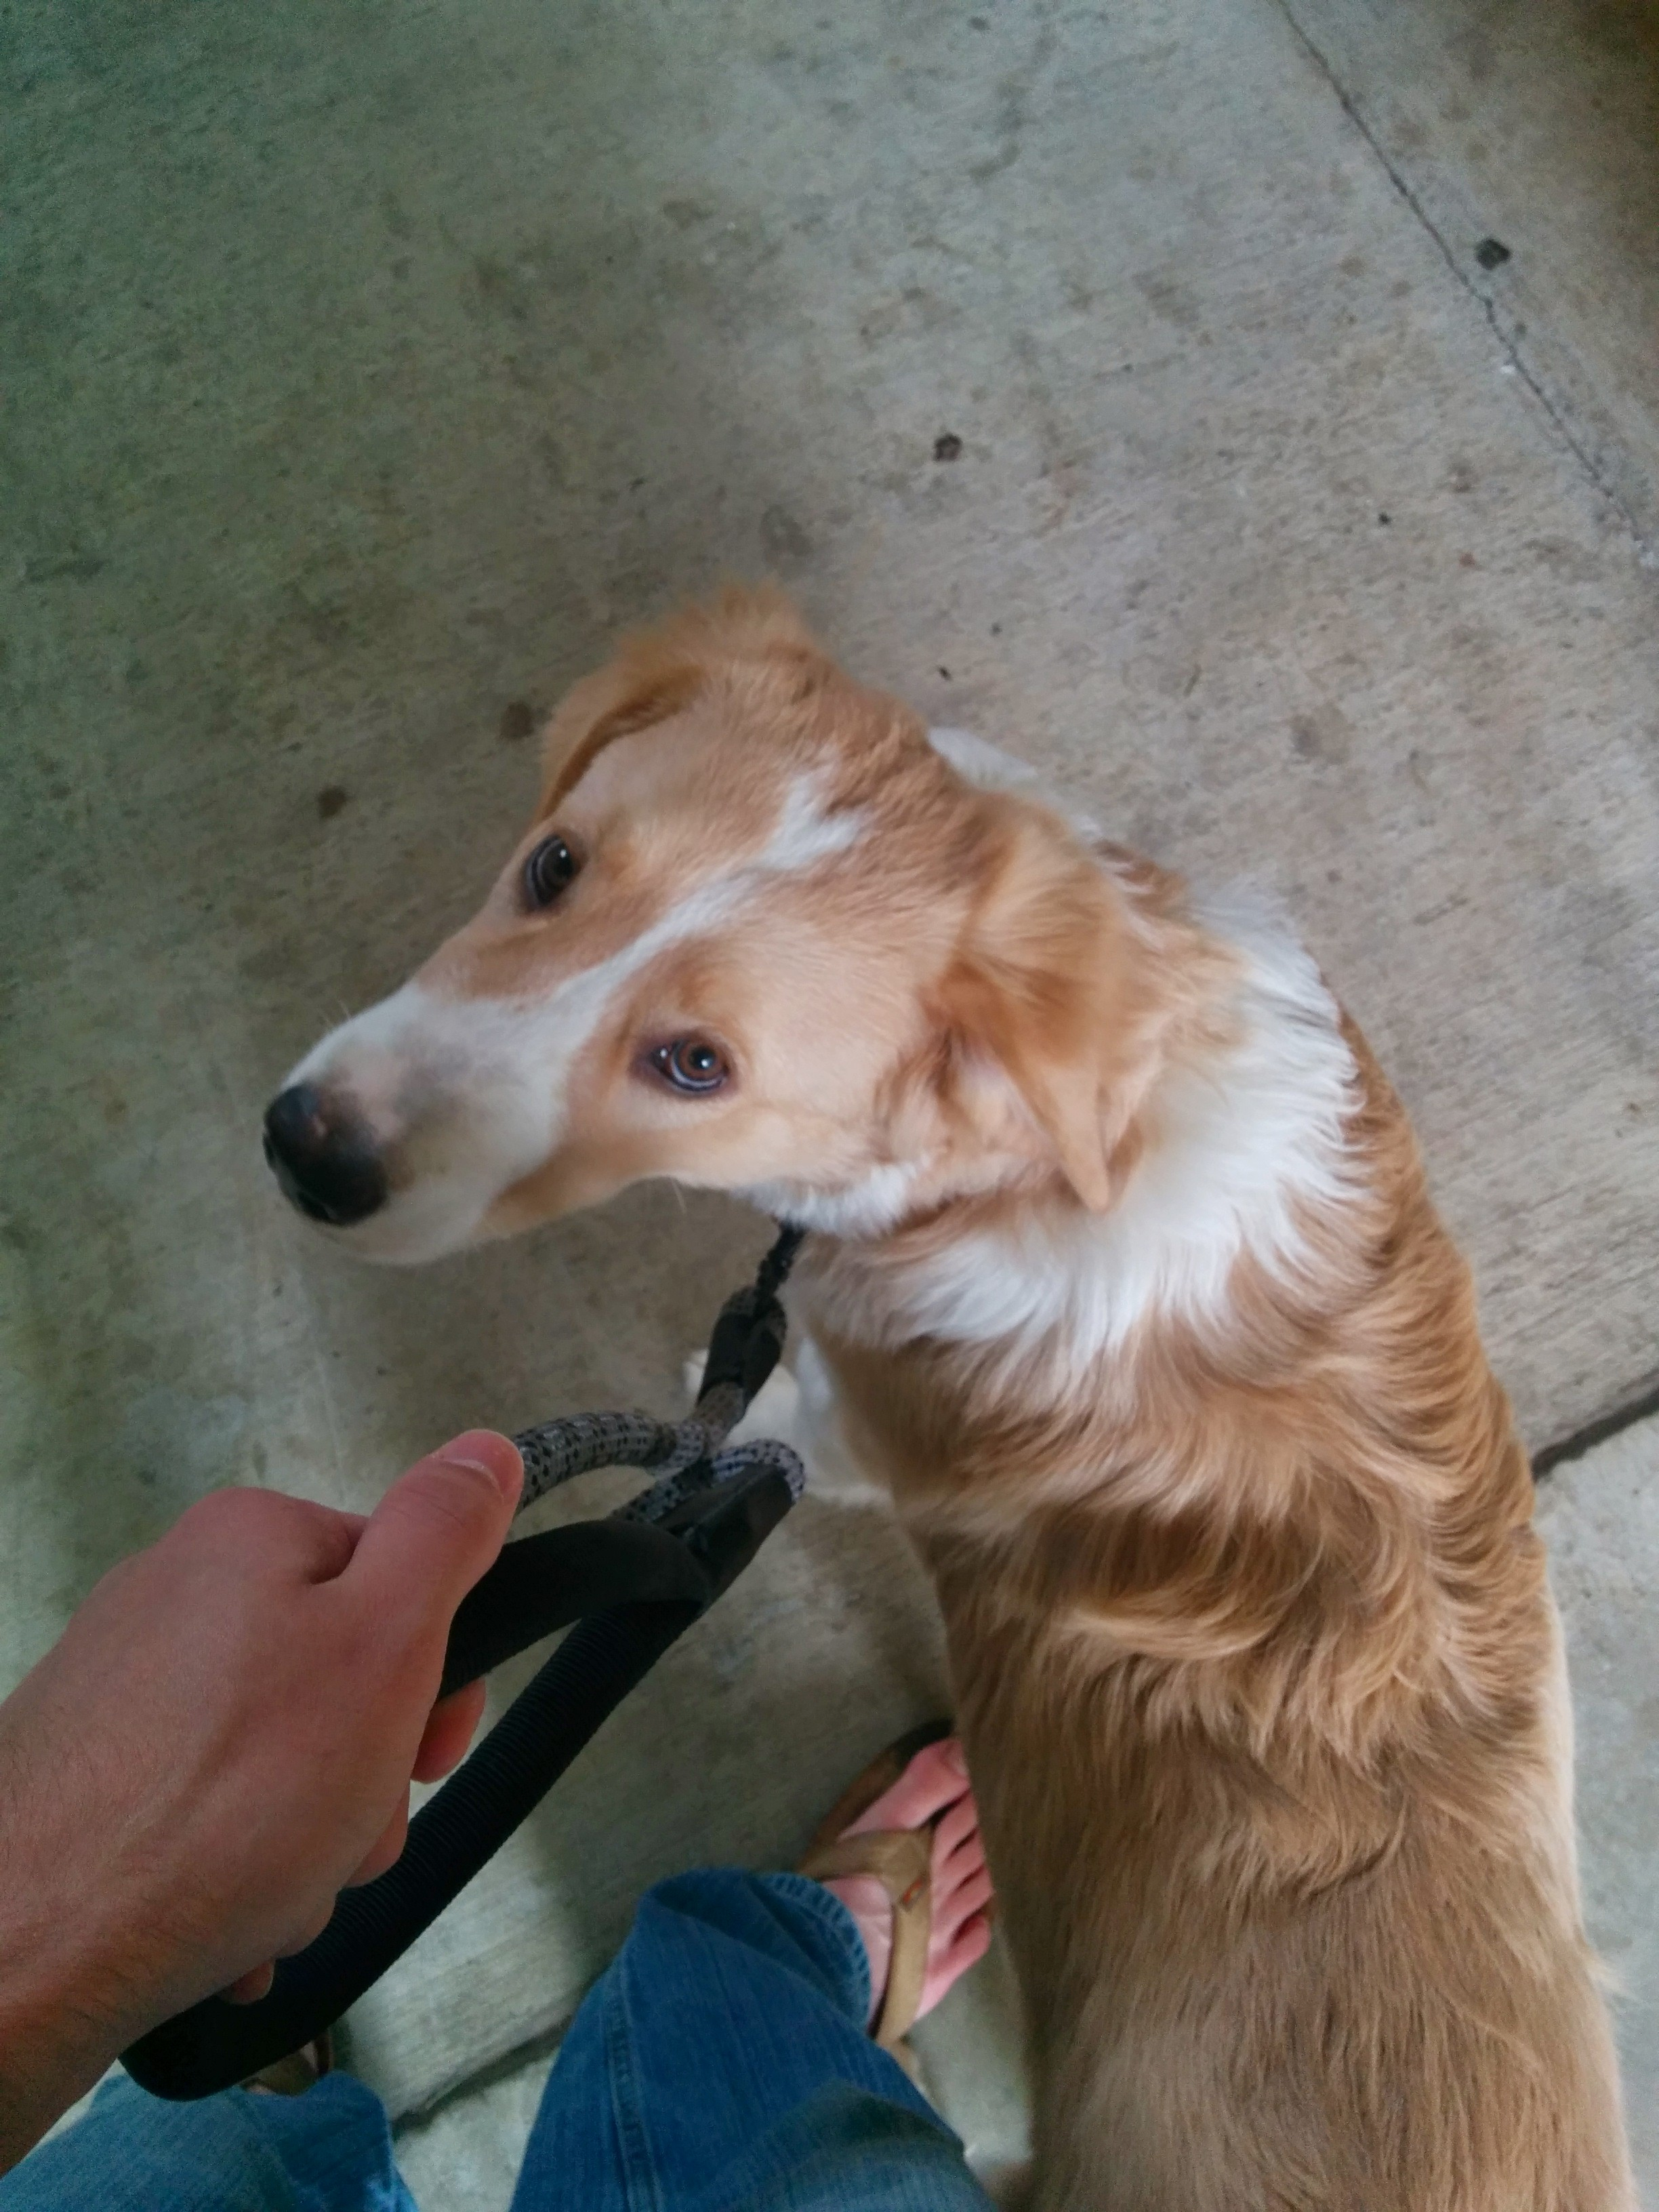
\includegraphics[width=.35\textwidth]{./images/how_to/walk_max/walking_max.jpg}
    \caption{Maxwell being walked at the correct leash length.}
    \label{fig:walking_max}
\end{figure}

\begin{figure}[H]
    \centering
    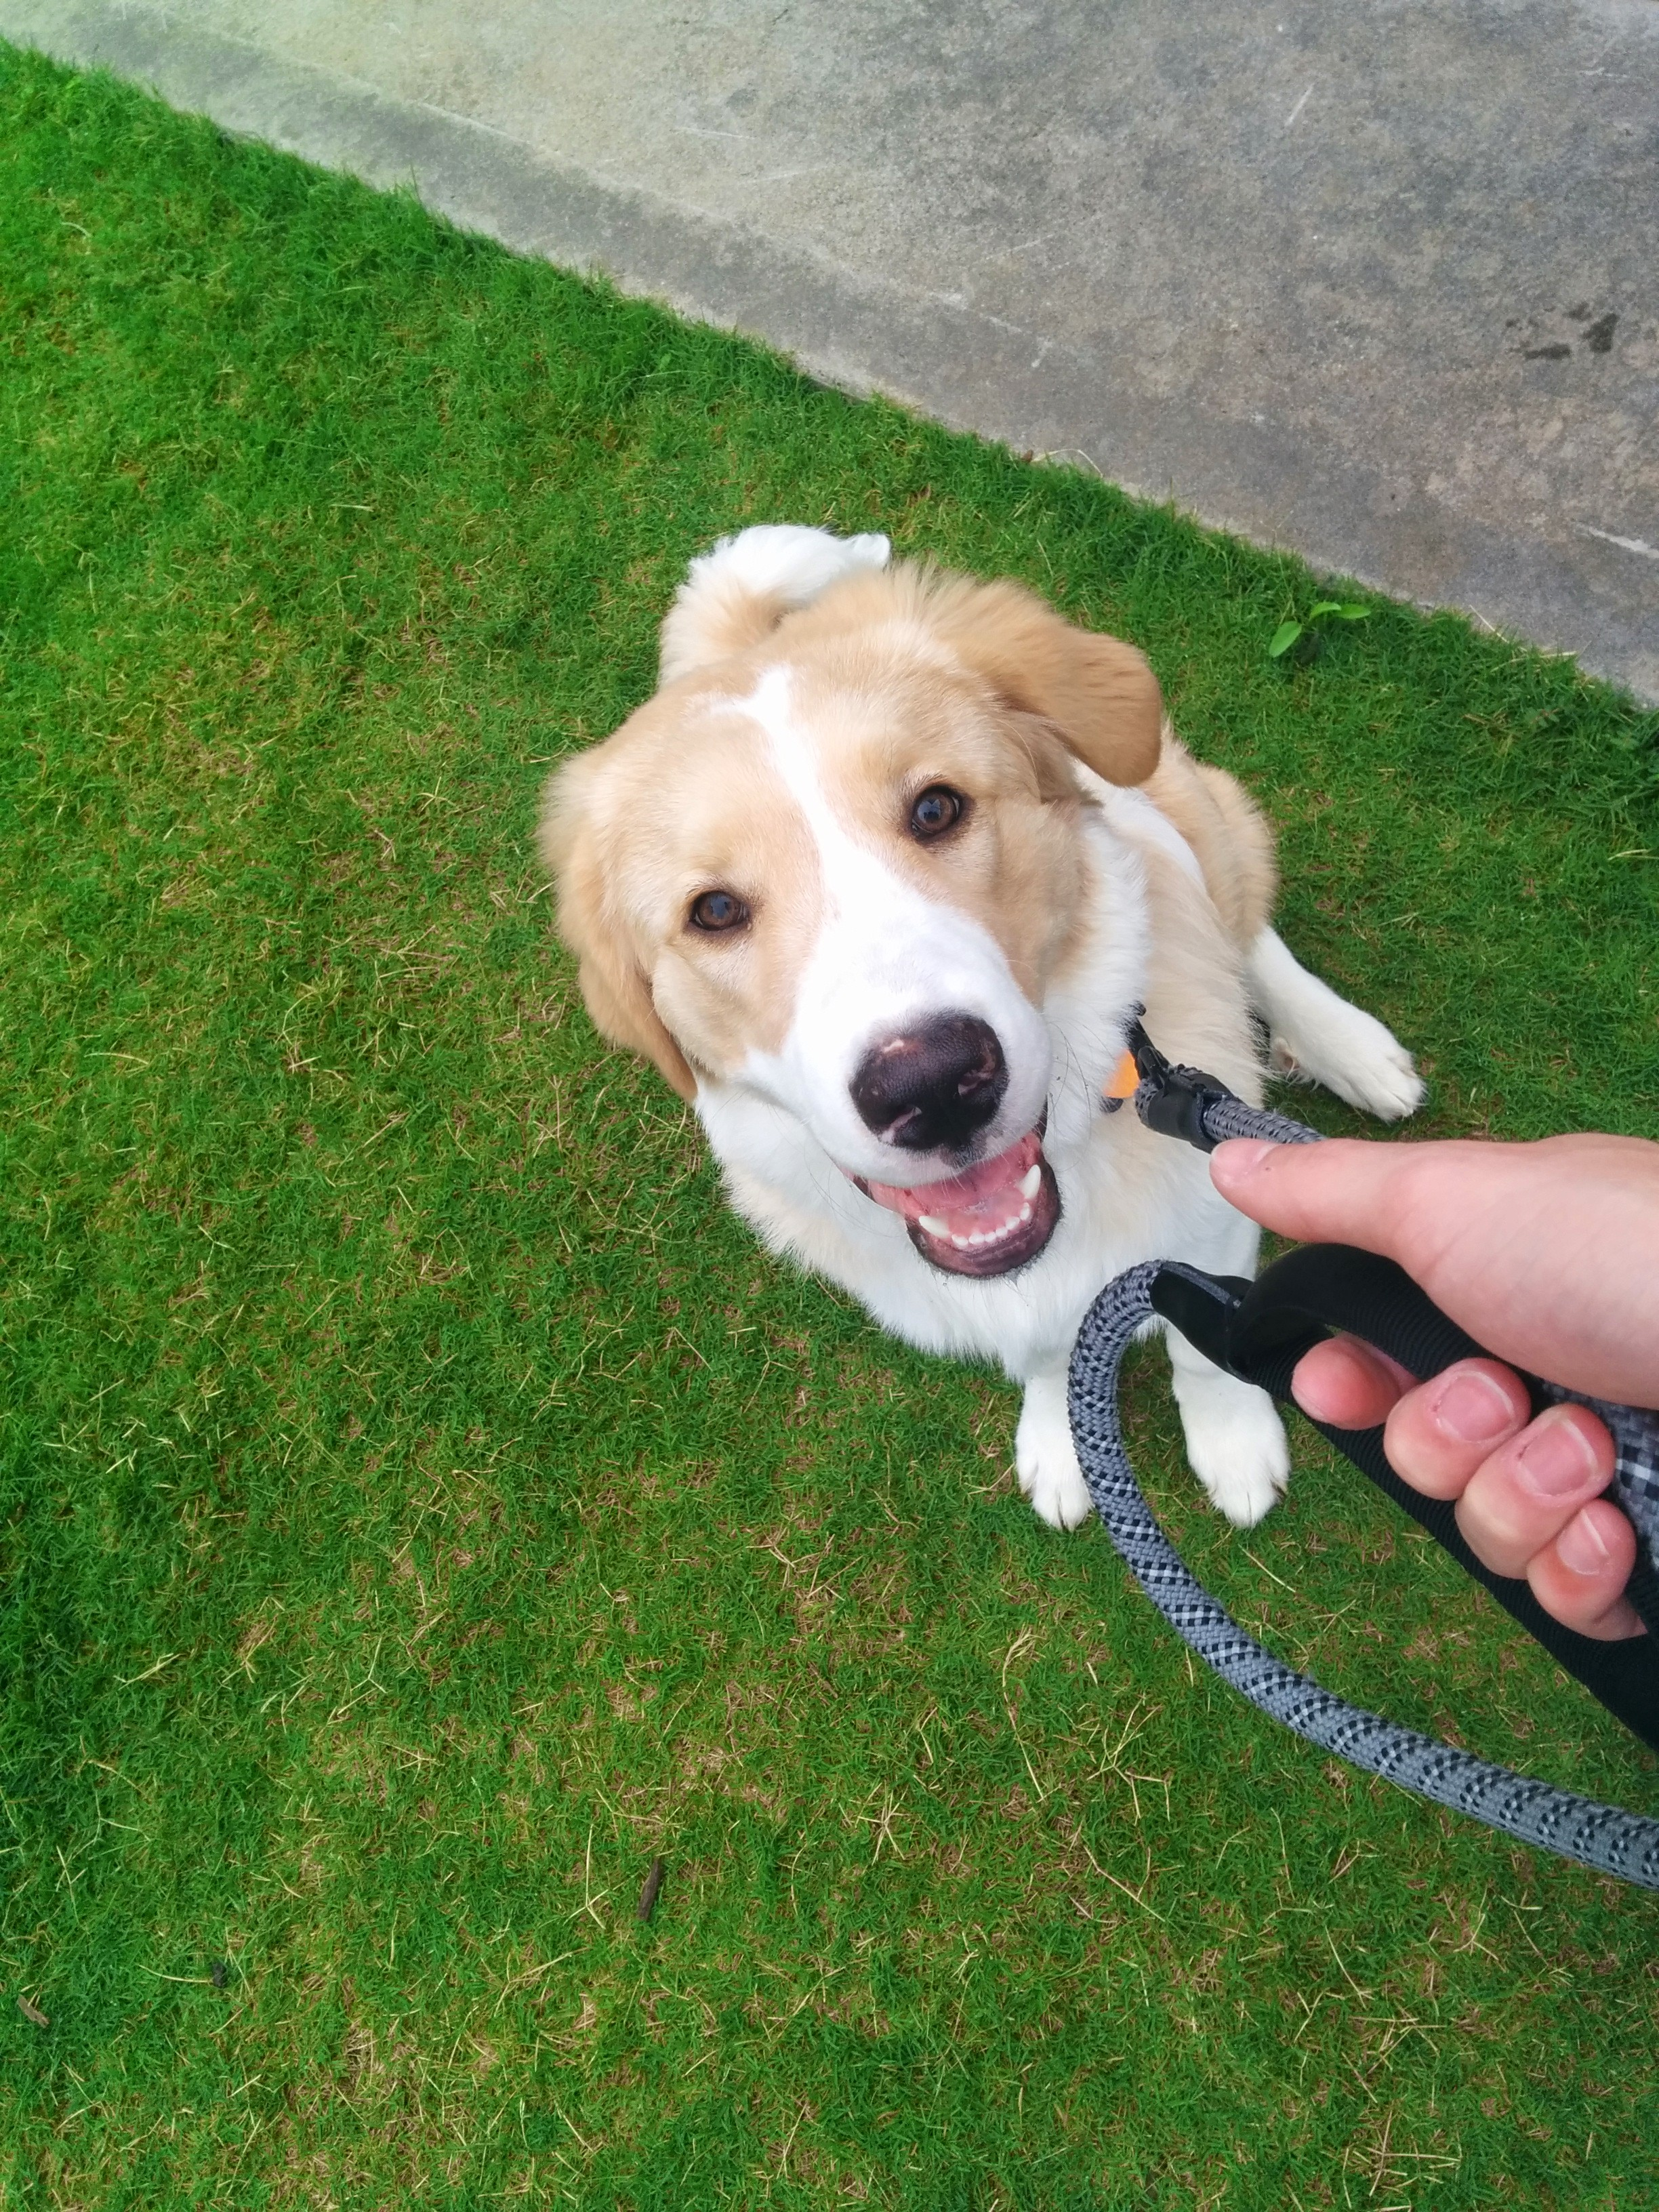
\includegraphics[width=.35\textwidth]{./images/how_to/walk_max/short_leash.jpg}
    \caption{Maxwell being walked at the correct leash length.}
    \label{fig:short_leash}
\end{figure}

\subsection{How to clean up an accident}
\begin{enumerate}\label{itm:how_to_clean_accident}
    \item Identify the spot where Max has gone
    \item Mark off the area, and put Max away
    \item Get the peepee solution, and paper towels from his bag
    \item Get a trashcan or other recepticle for the soaked paper towels
    \item Soak up the accident with the paper towels (note: this will be disgusting)
    \item When the paper towels come away "generally" dry, open the peepee solution to "spray"
    \item Spray the solution around the area so that it soaks into the carpet
    \item Let sit for 3-5 minutes
    \item Scrub the solution into the carpet with paper towels
    \item Soak up the excess solution with paper towels
    \item Repeat as necessary
\end{enumerate}

\subsection{How to put on the Easy Walk Harness}
\begin{enumerate}\label{itm:how_to_harness}
    \item See Fig~\ref{fig:harness_steps} on page~\pageref{fig:harness_steps}.
    \item Place the harness on the floor with the dark towards you, and
        the light side towards Max.
    \item Connect the dark band around Max's neck and chest, attaching the clasp
        in the back behind his shoulders.
    \item Run the light side underneath Max's underside and attach the clasp to
        on Max's right side shoulder.
    \item Attach the leash to the front ring on Max's chest.
    \item When walking Max with this harness, maintain a loose leash.
    \item Make sure the harness is snug and secure.
    \item Make sure that the harness' "O" rings reside on Max's shoulders where
        his legs connect to his body.
\end{enumerate}

\begin{figure*}
    \subfigure[1]{
        \label{fig:flat_harness}
        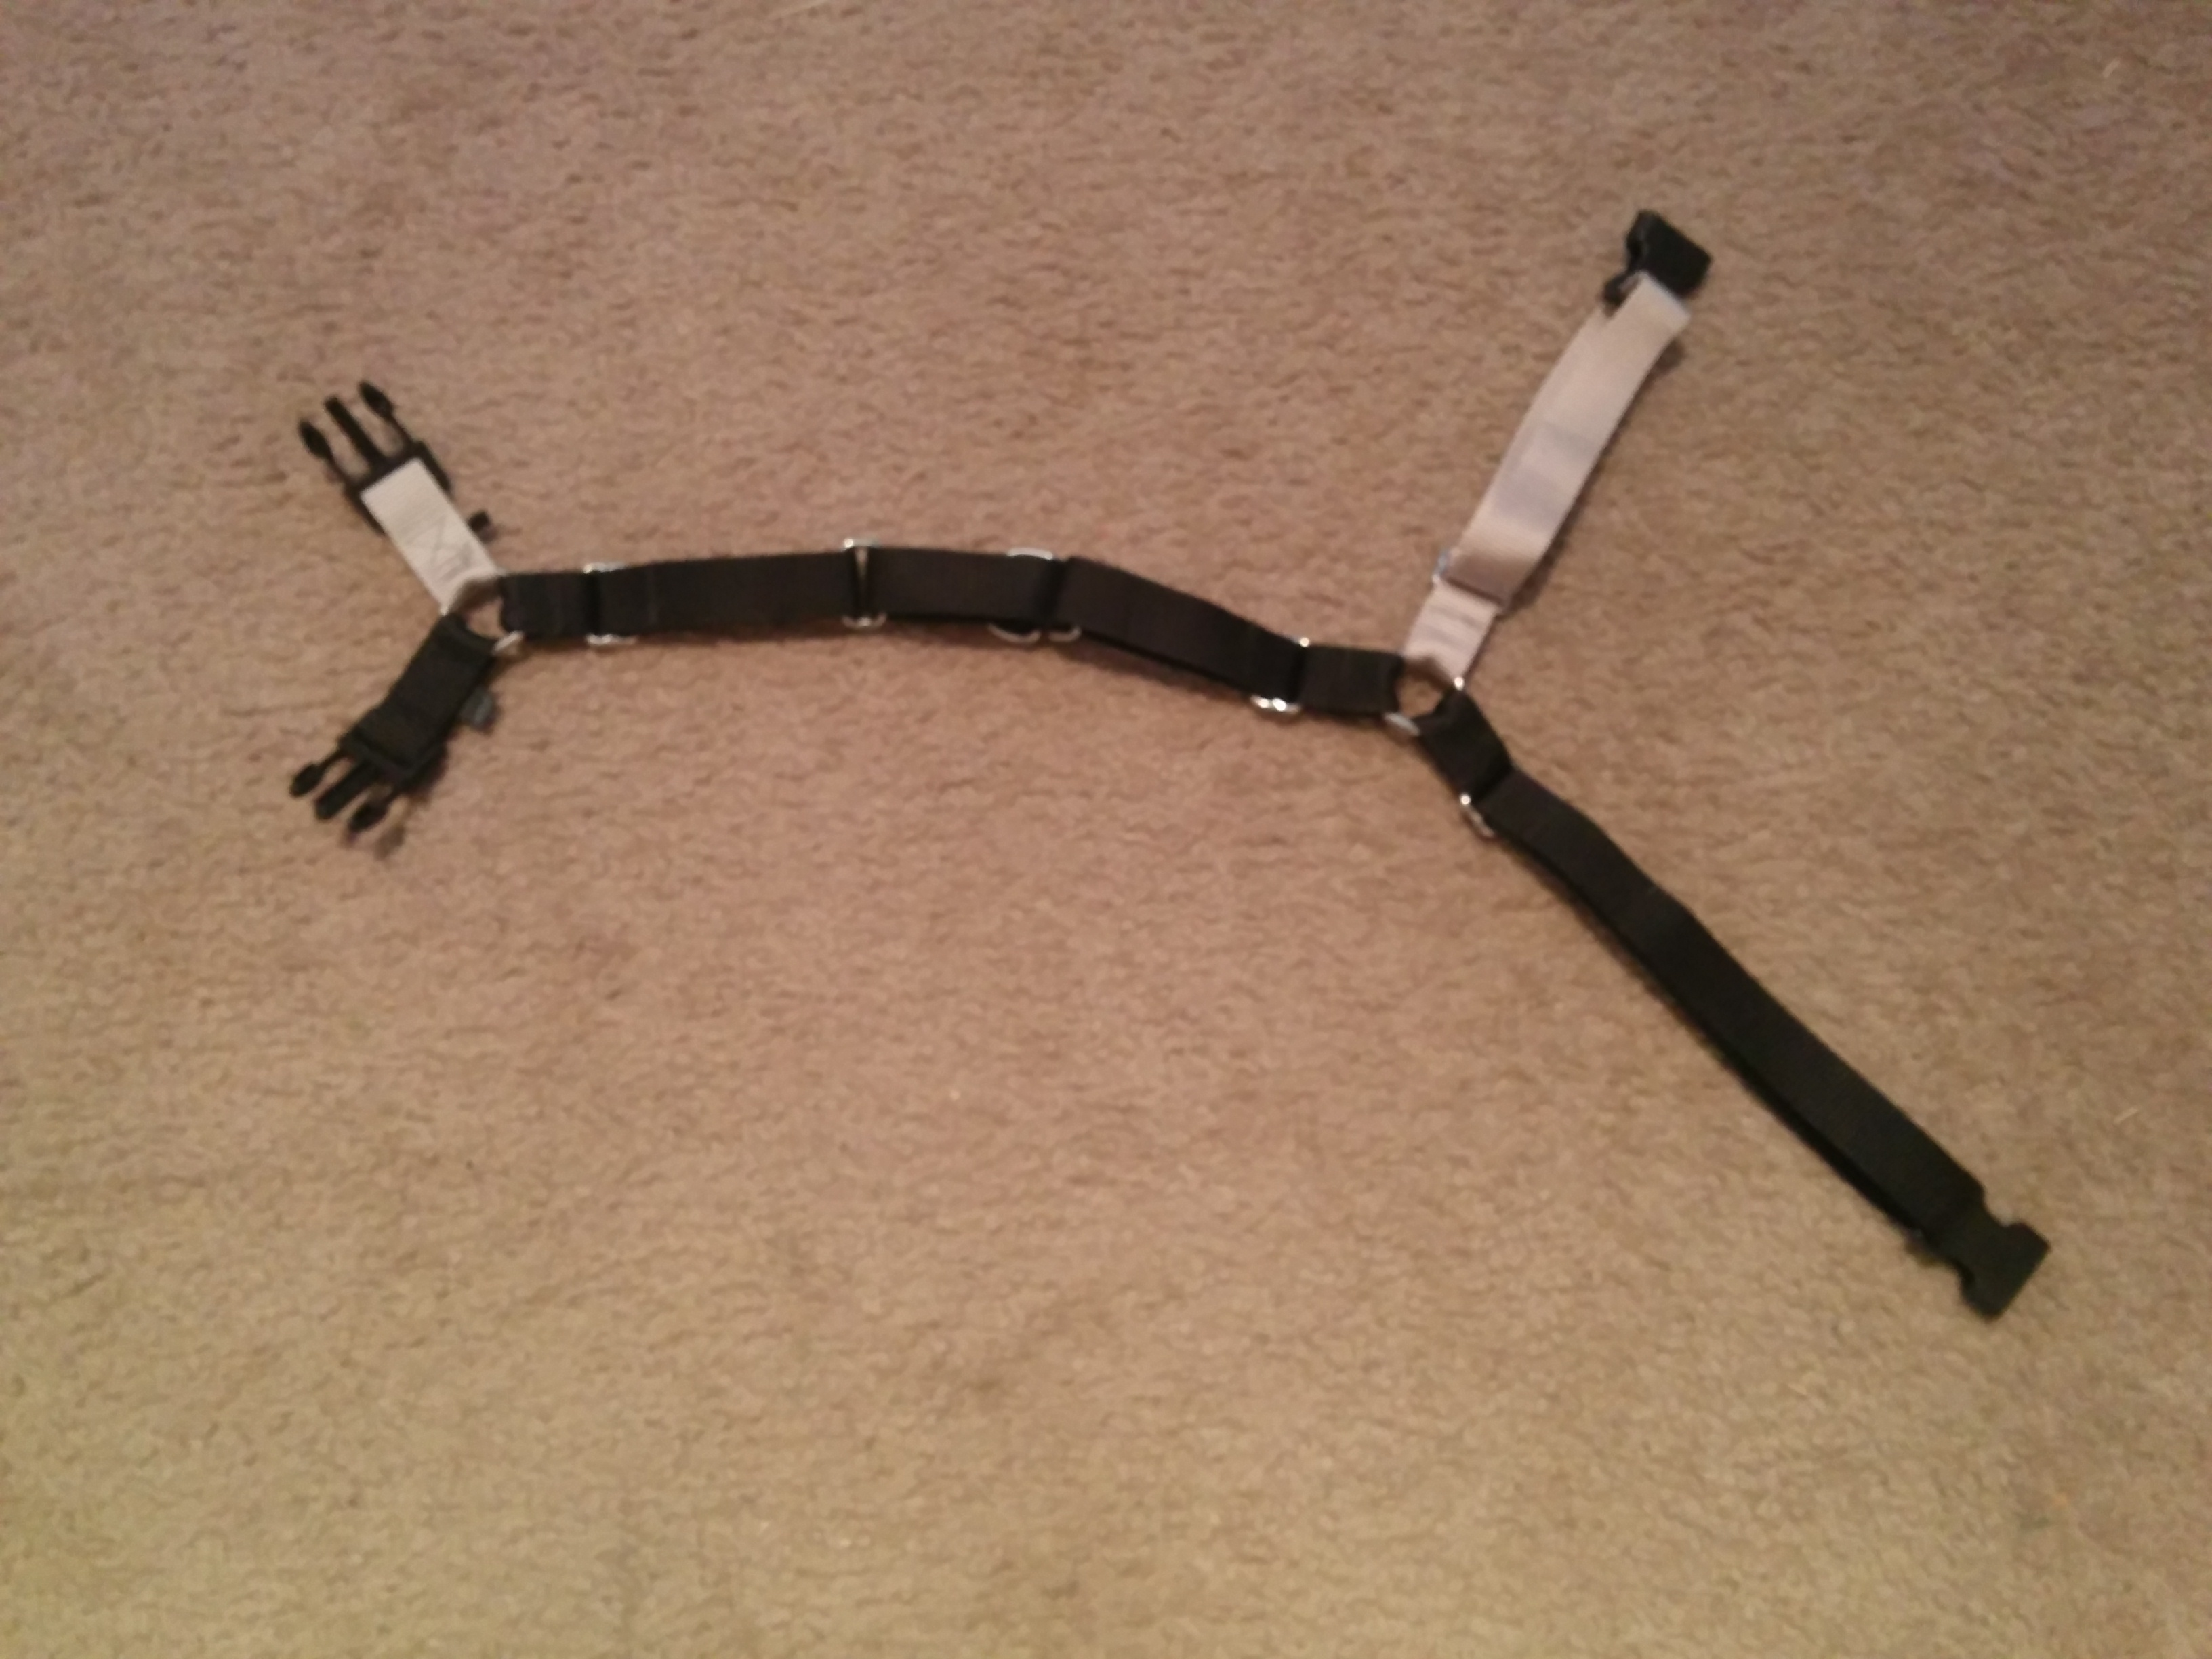
\includegraphics[width=0.35\textwidth]{./images/how_to/harness/flat_harness.jpg}
    }
    \hspace*{\fill}
    \subfigure[2]{
        \label{fig:dark_strap}
        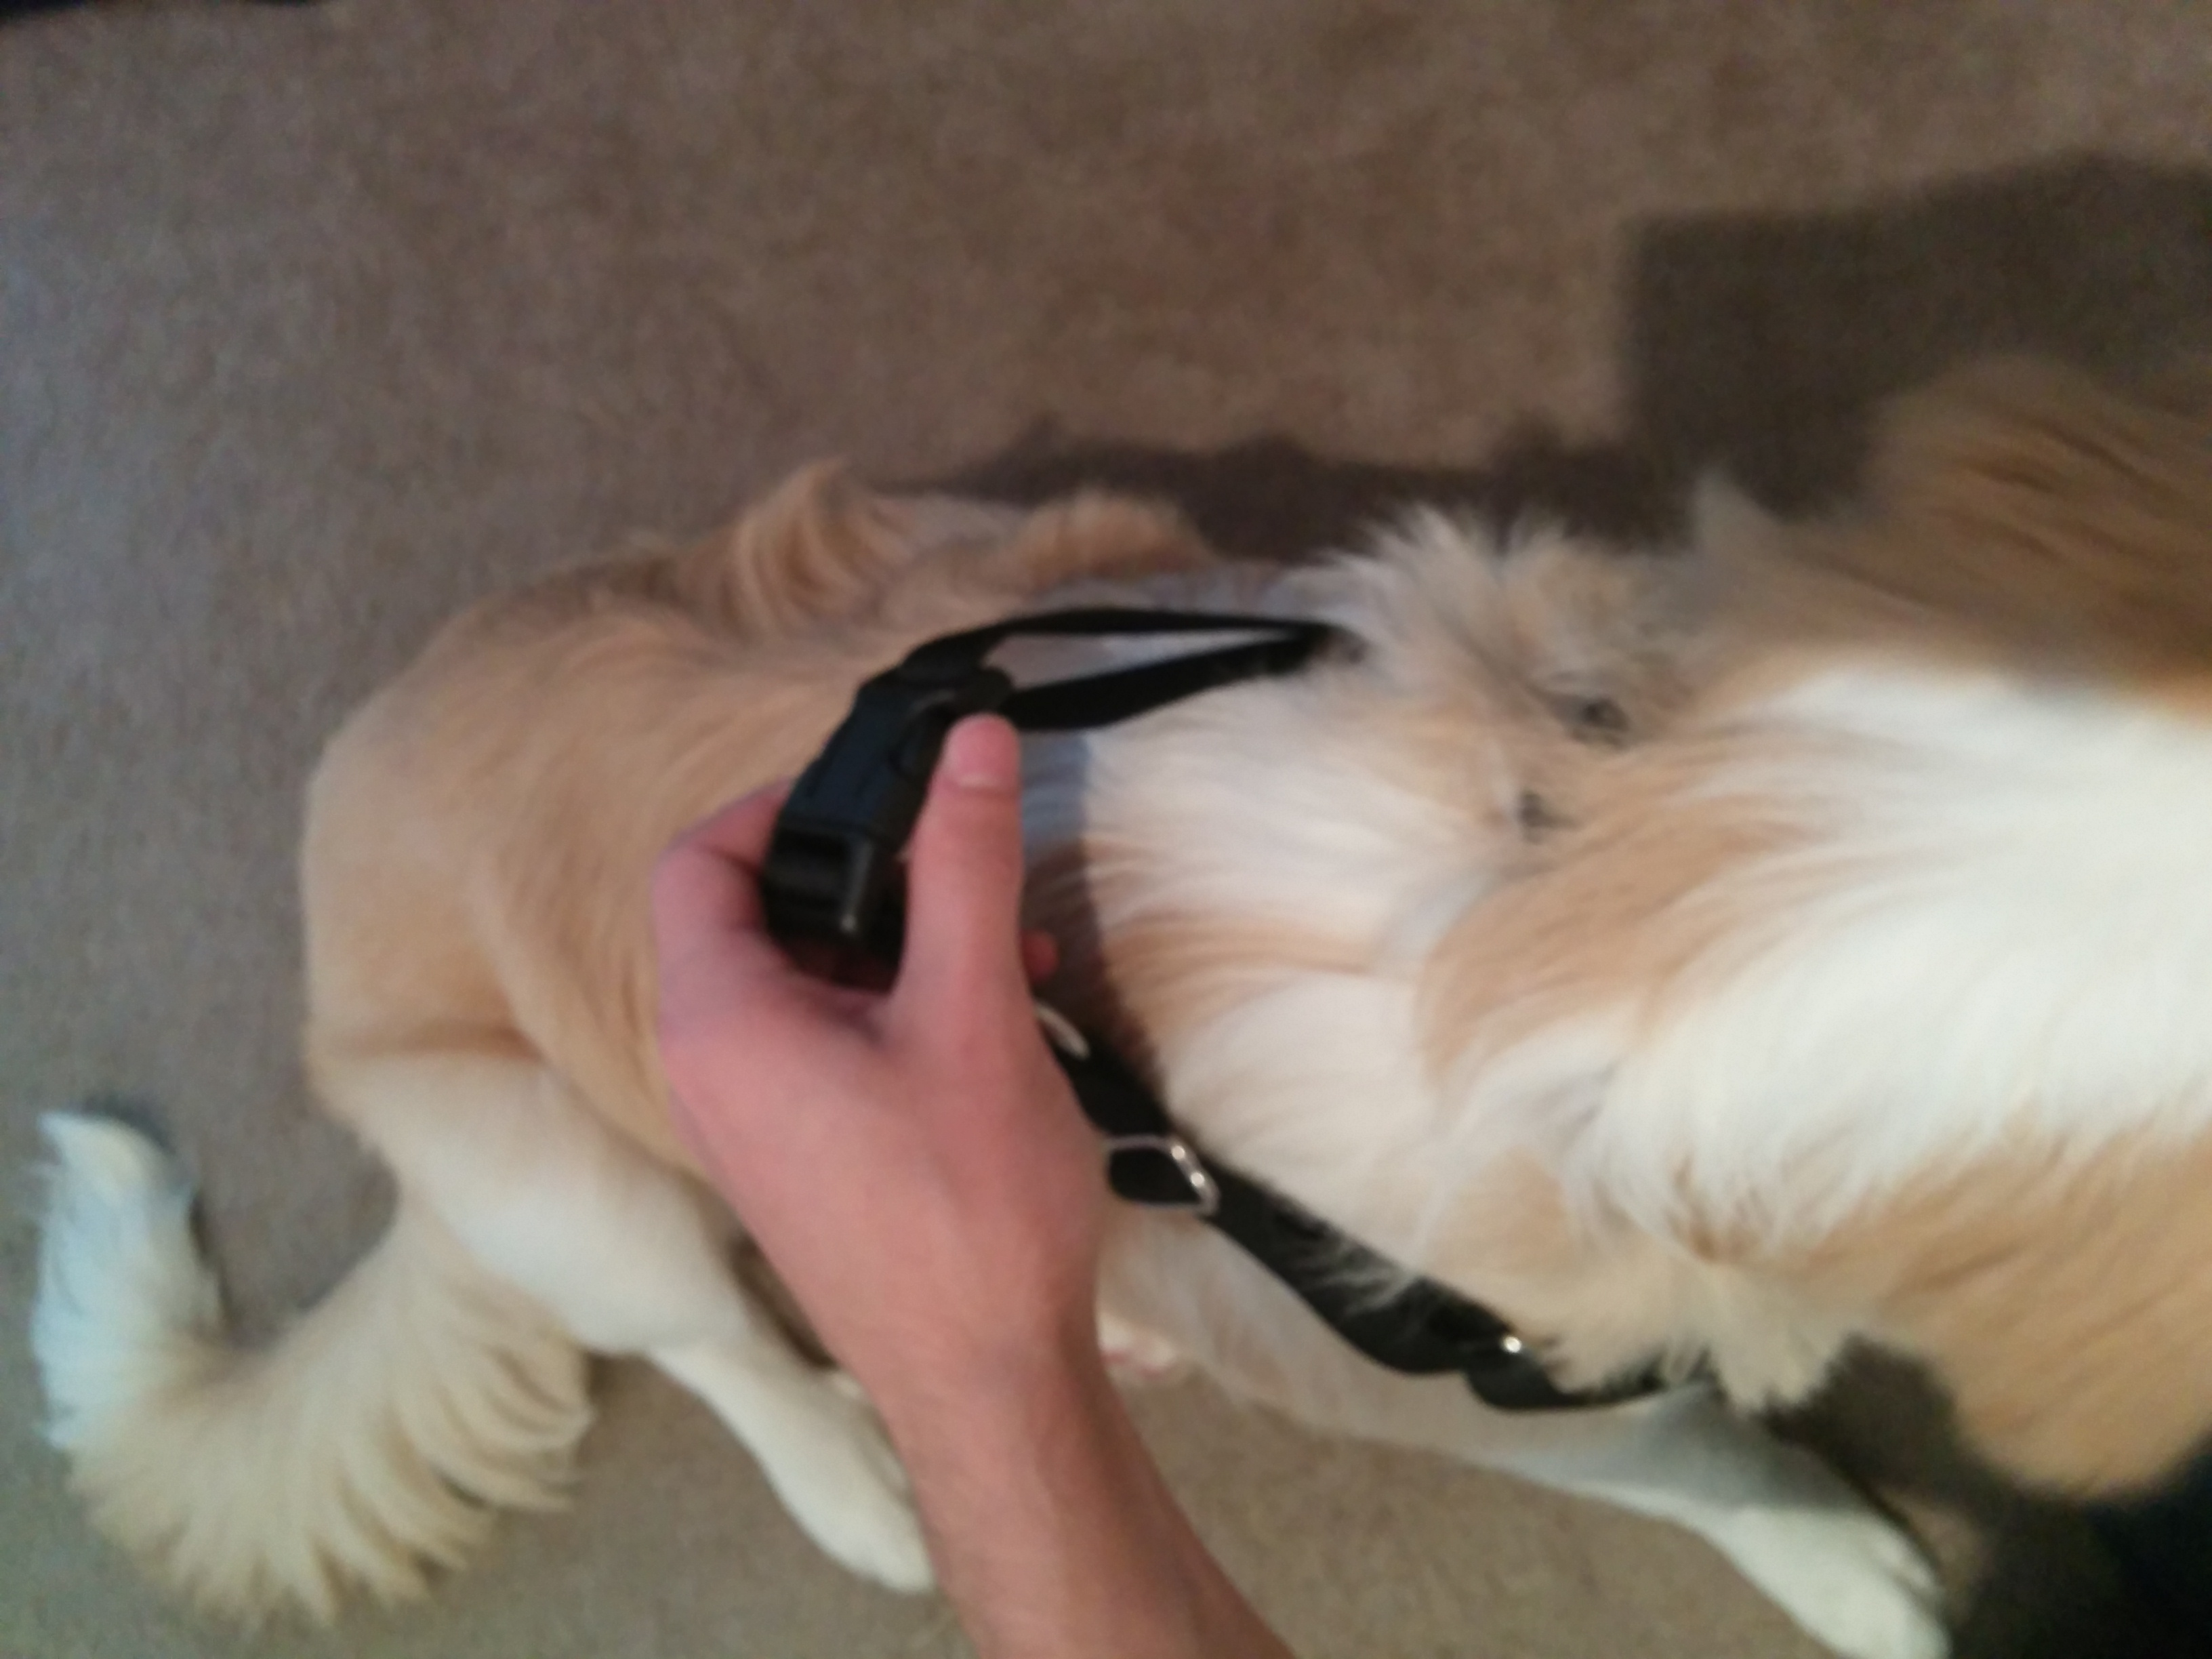
\includegraphics[width=0.35\textwidth]{./images/how_to/harness/dark_strap.jpg}
    }

    \\
    \subfigure[3]{
        \label{fig:light_strap}
        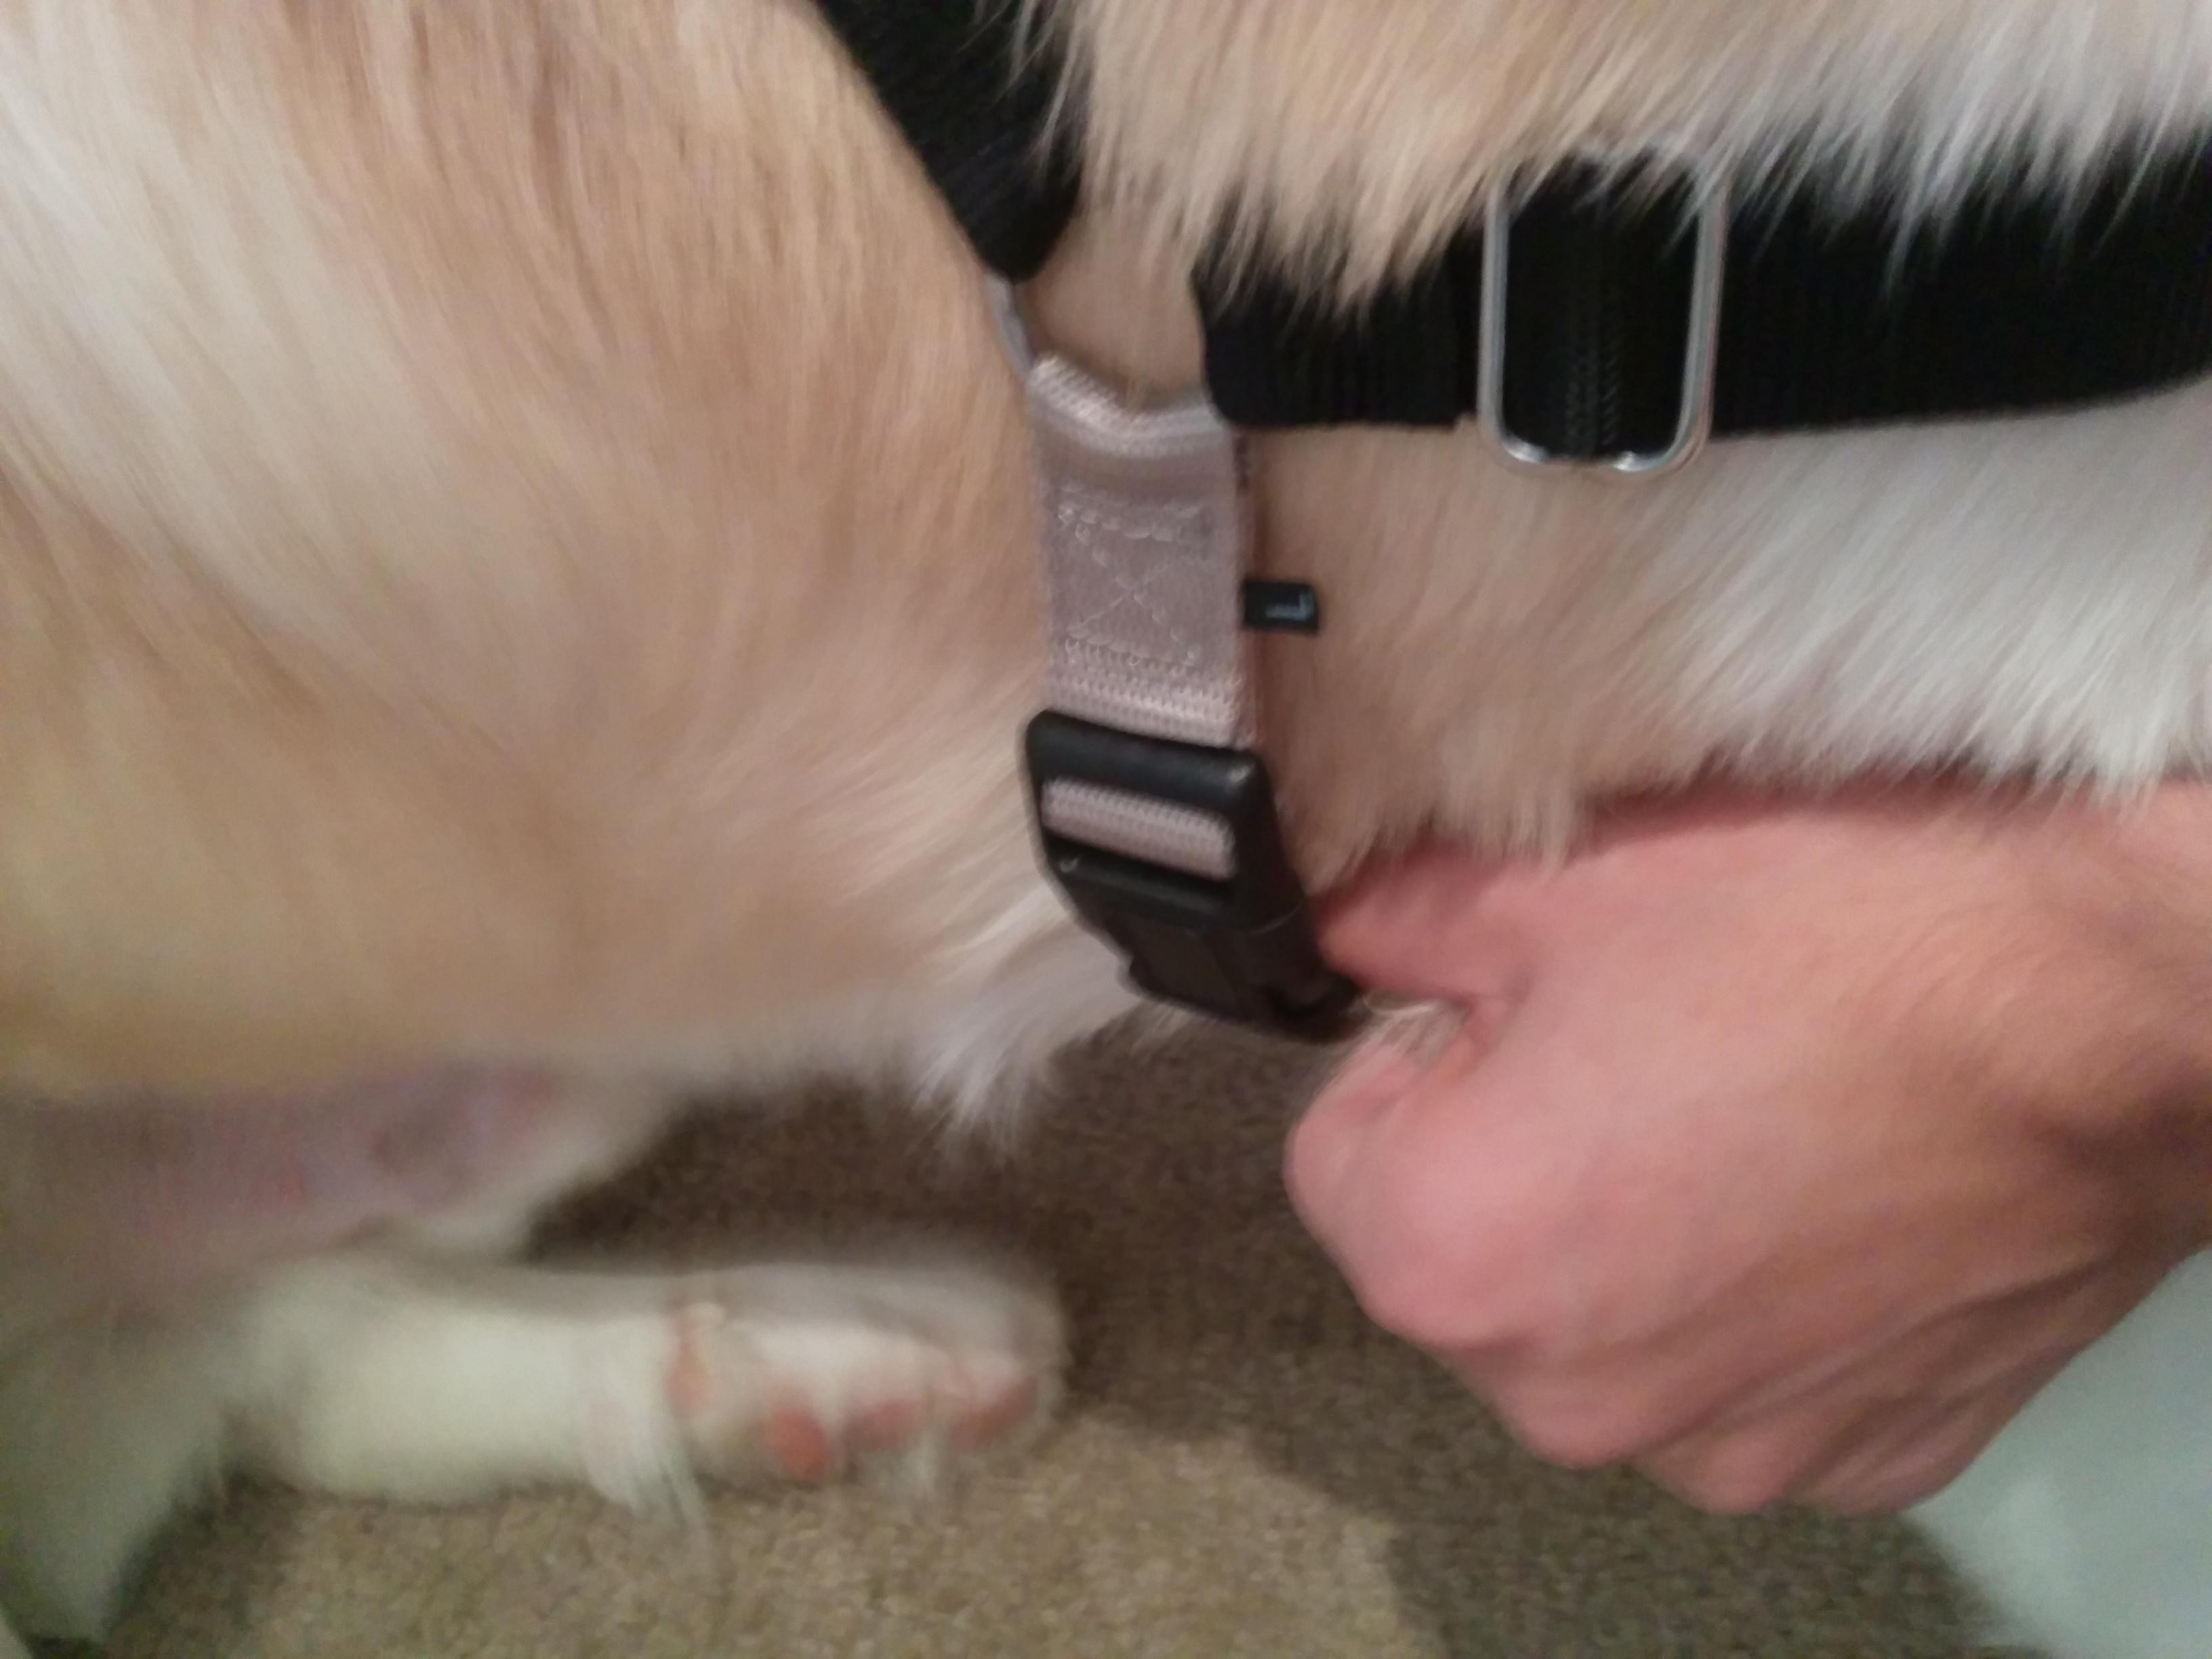
\includegraphics[width=0.35\textwidth]{./images/how_to/harness/light_strap.jpg}
    }
    \hspace*{\fill}
    \subfigure[4]{
        \label{fig:leash_attach}
        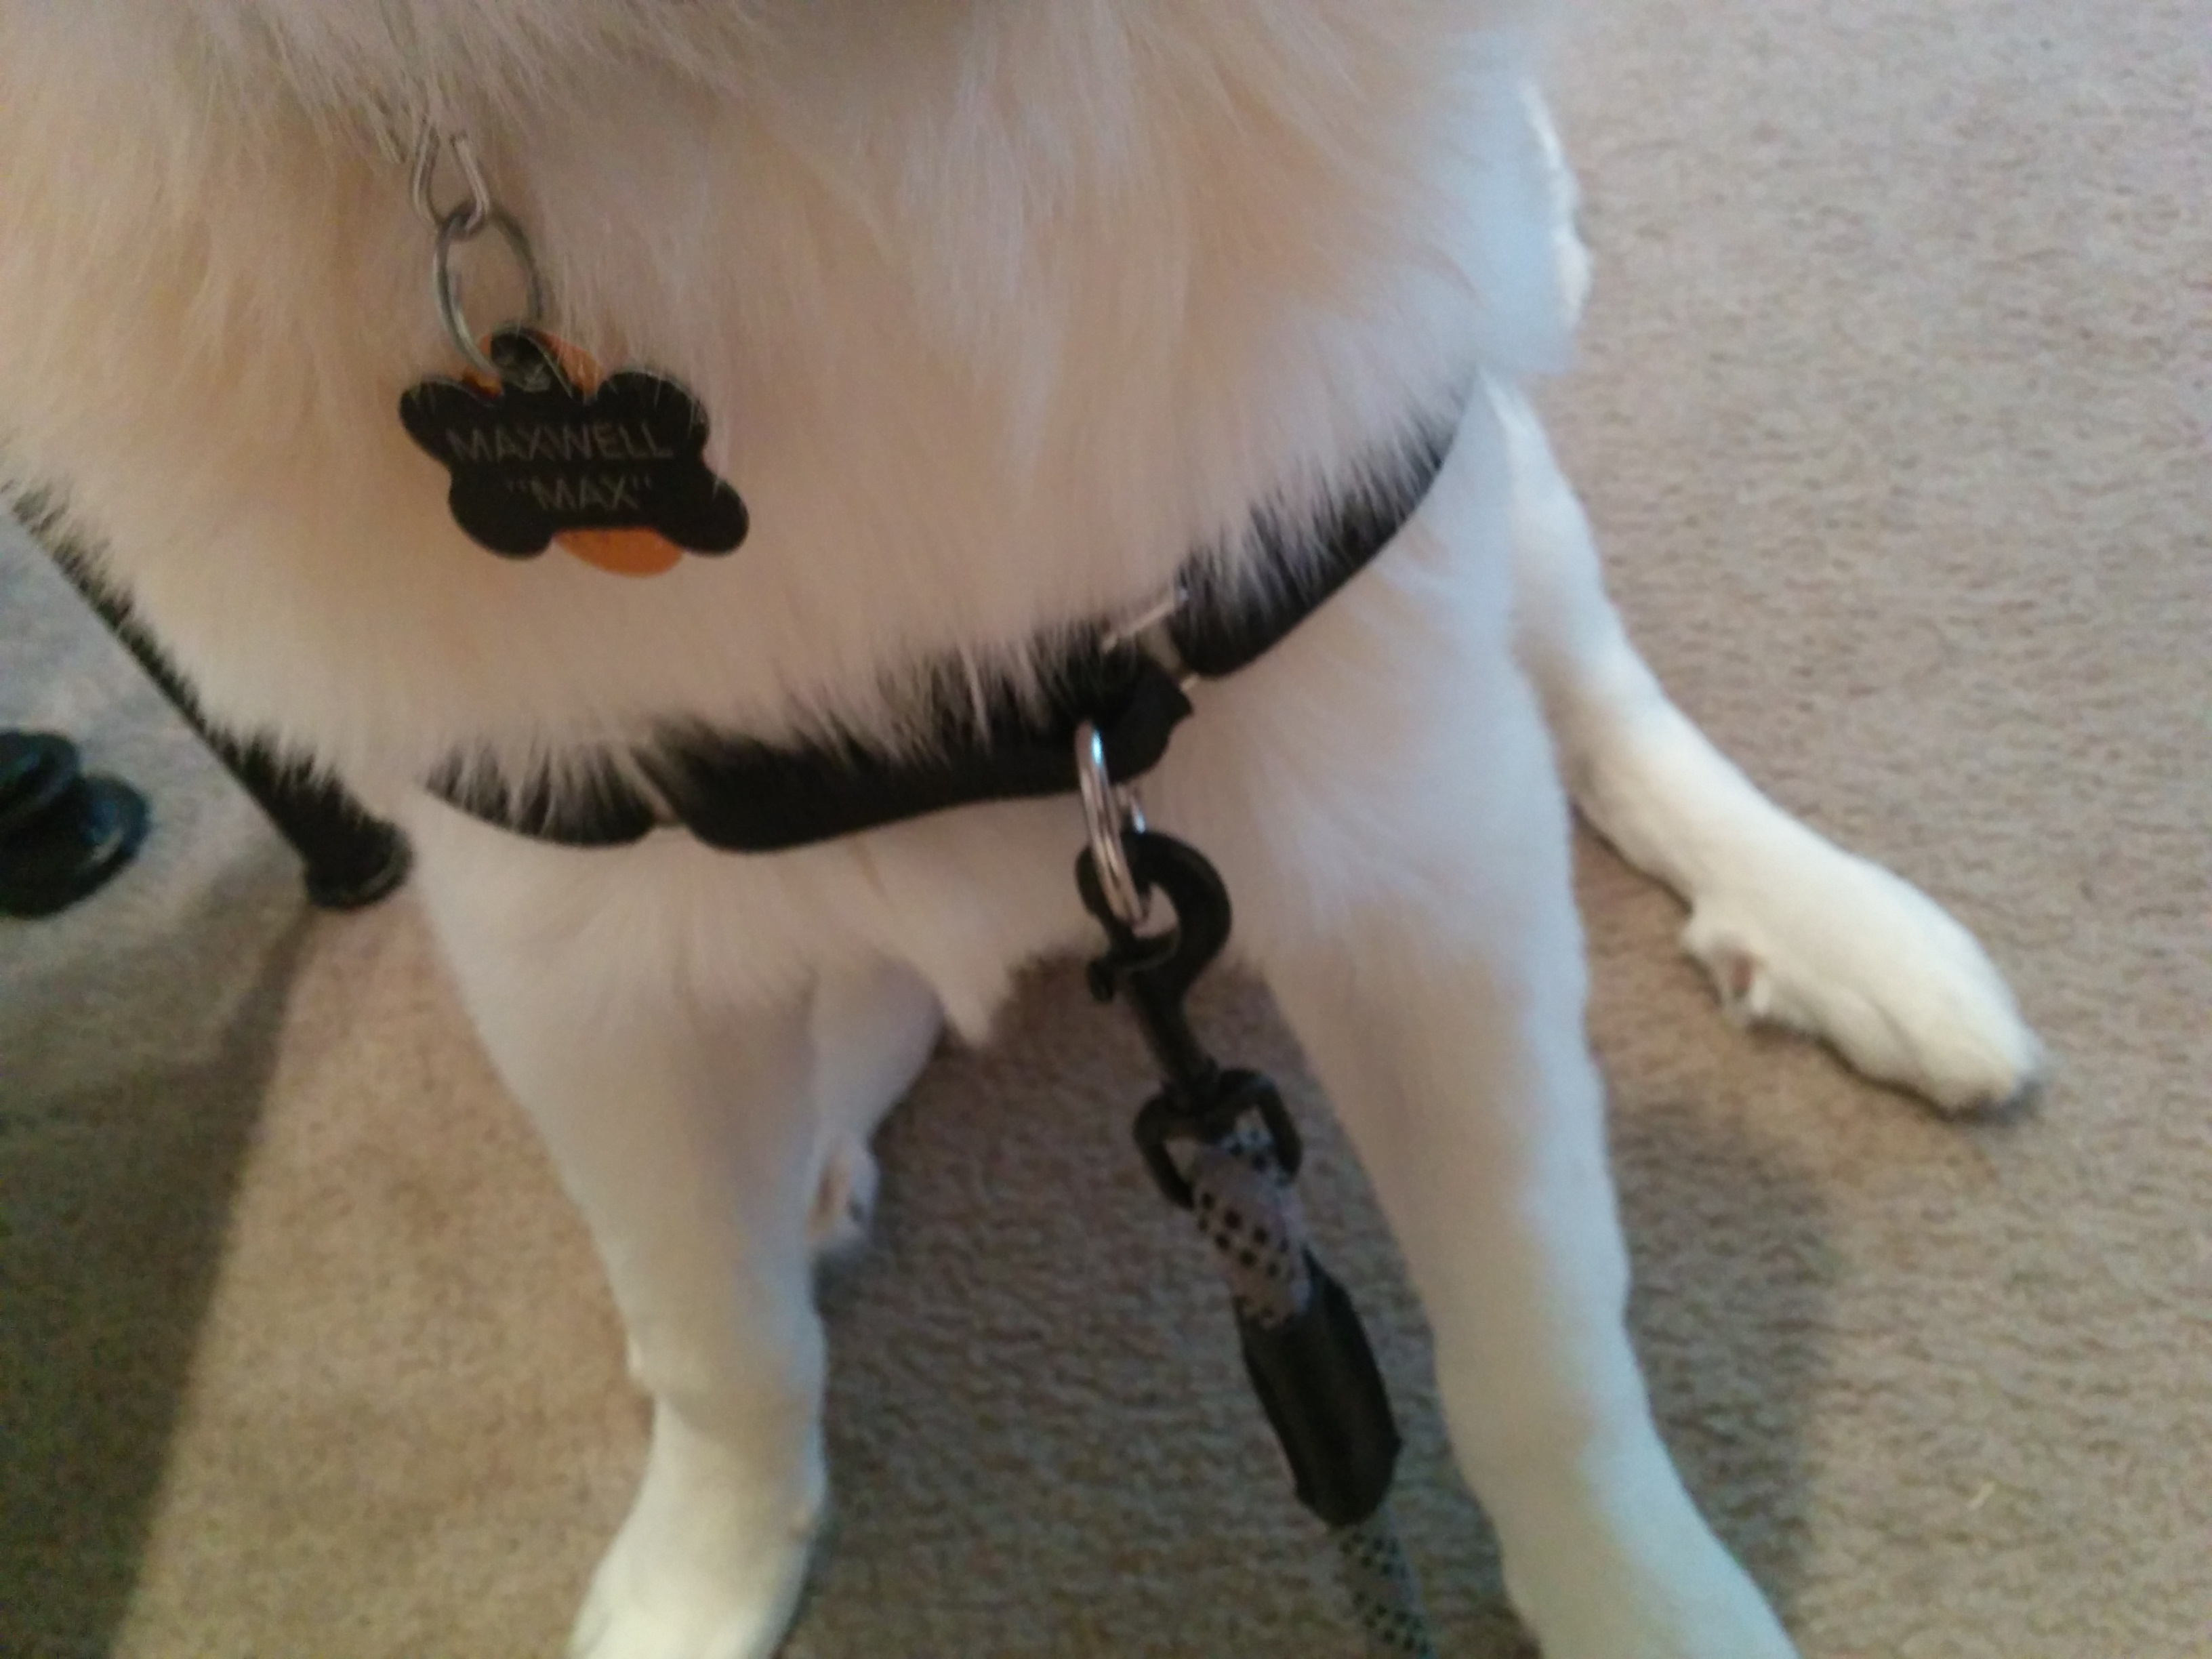
\includegraphics[width=0.35\textwidth]{./images/how_to/harness/leash_attached.jpg}
    }

    \\
    \subfigure[5]{
        \label{fig:harness_walk}
        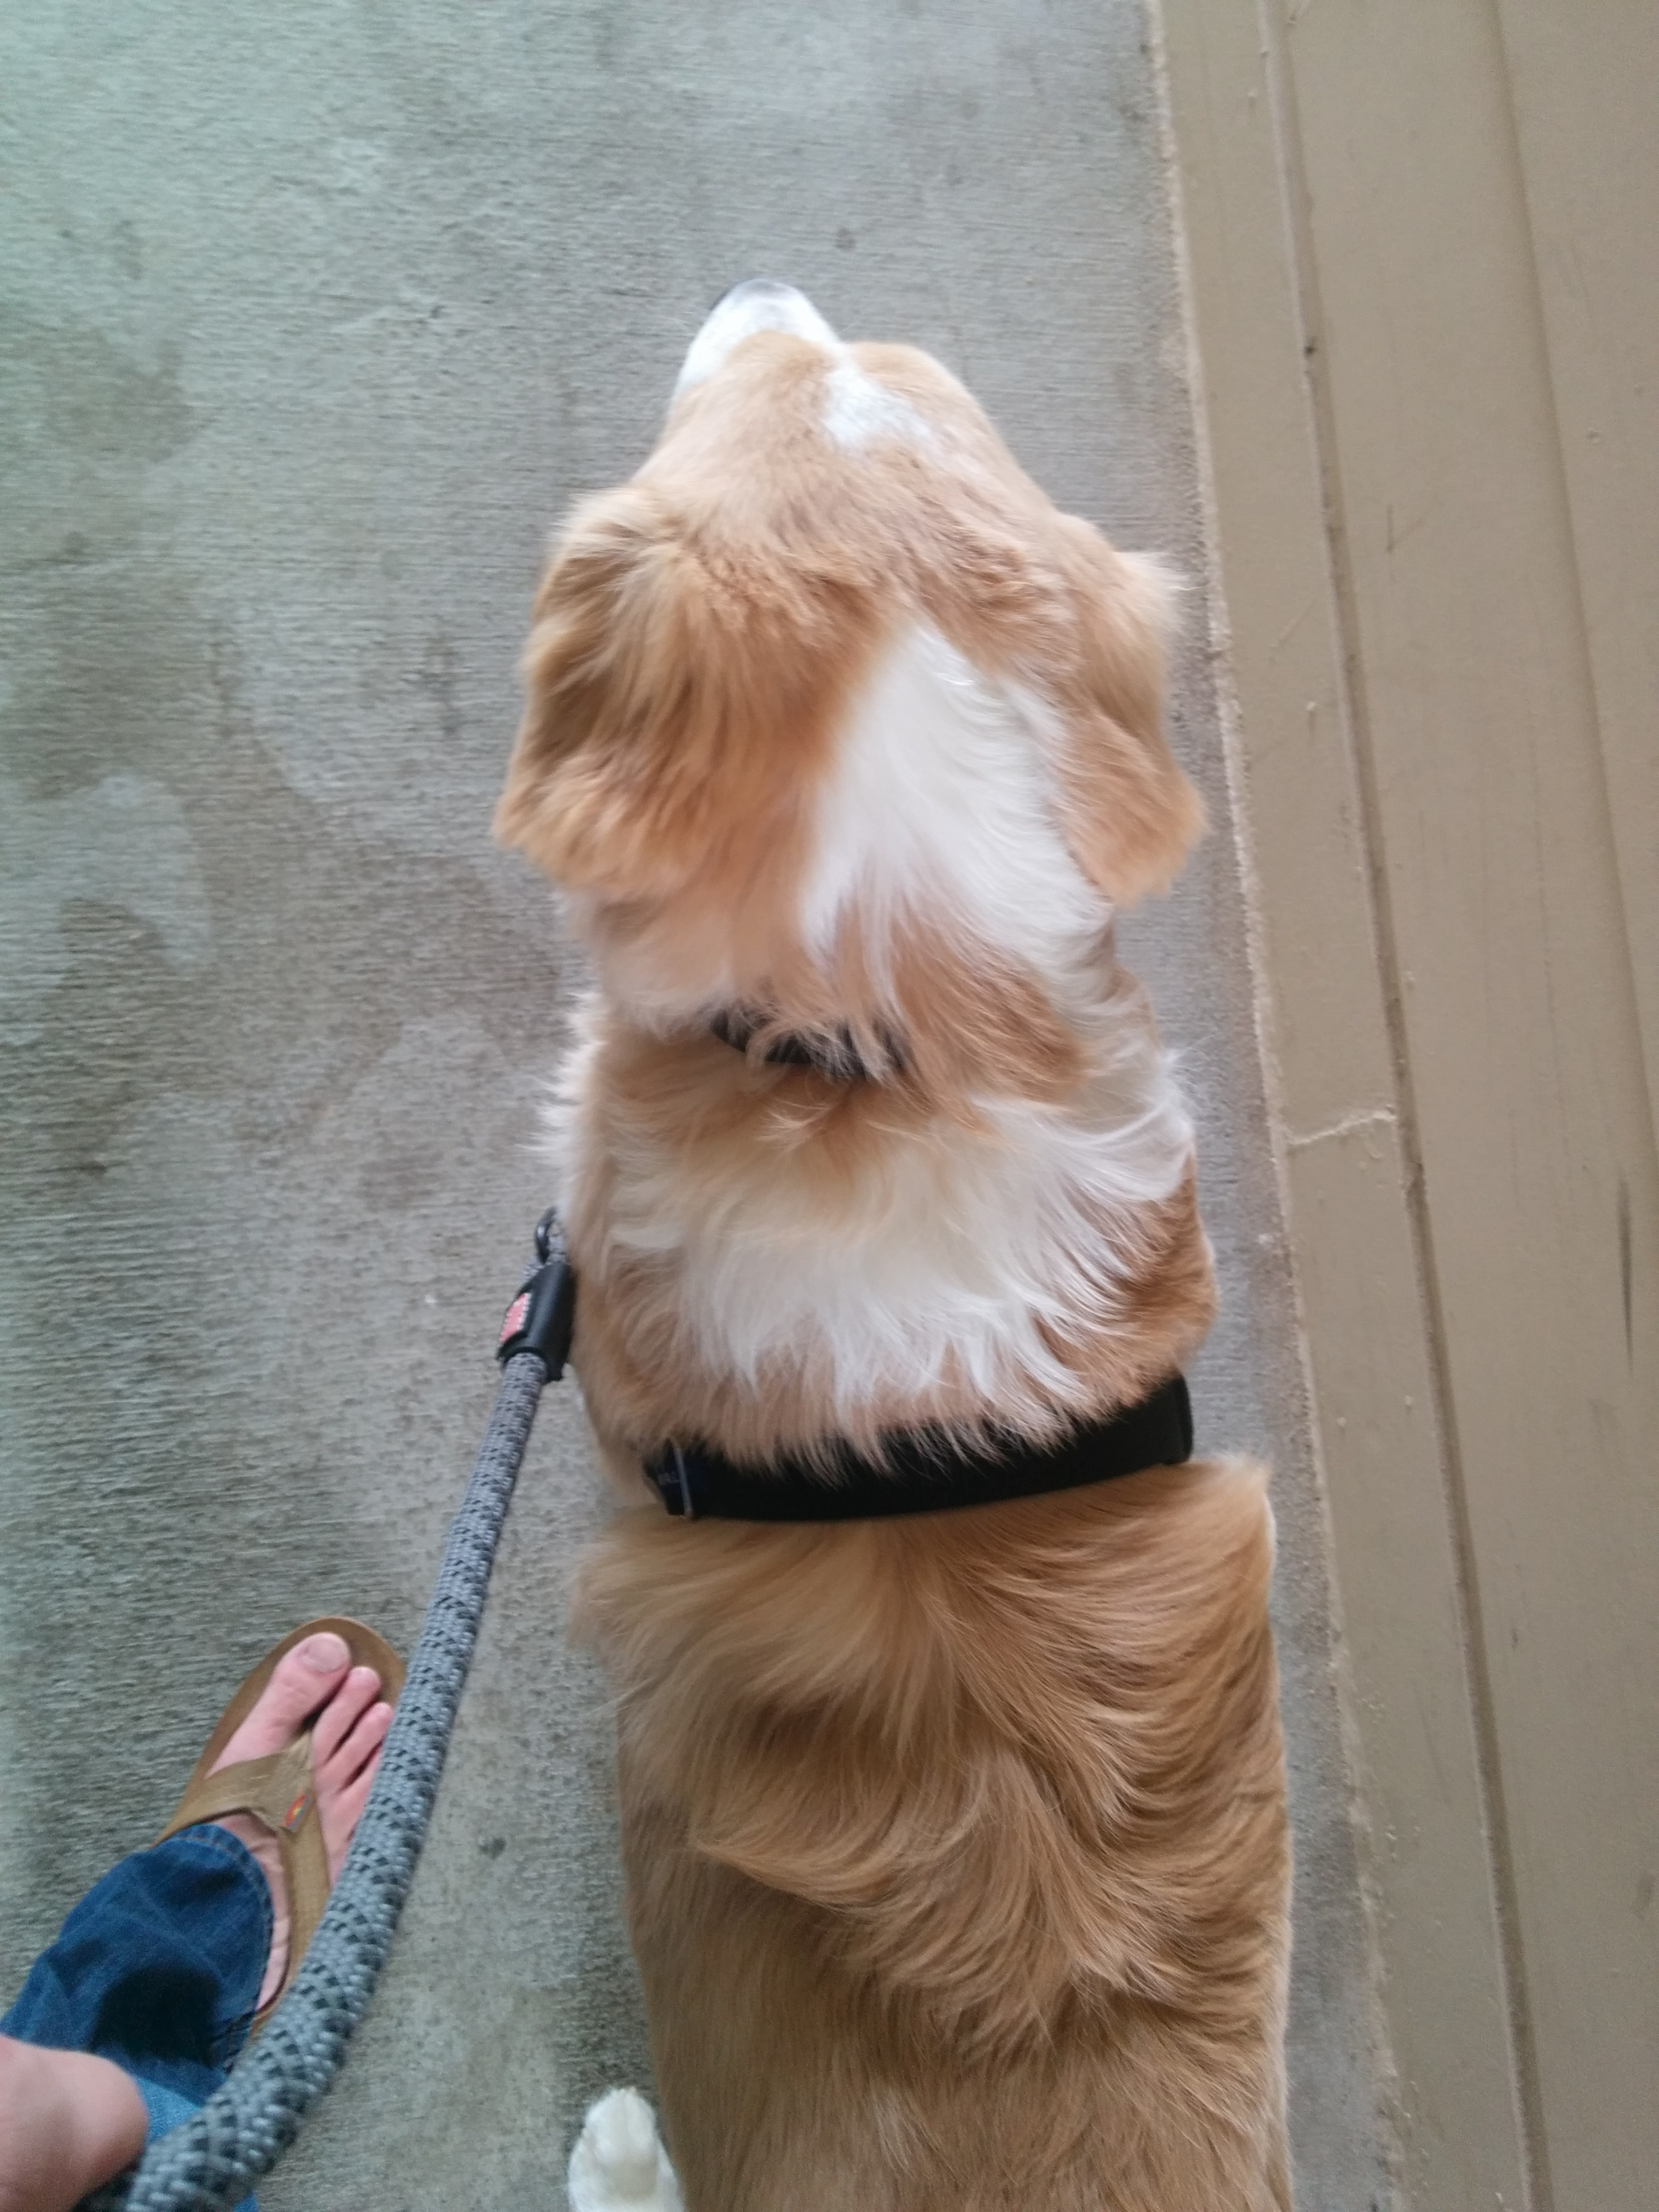
\includegraphics[width=0.35\textwidth]{./images/how_to/harness/harness_walk.jpg}
    }
    \caption{How to put on the Easy Walk Harness.}
    \label{fig:harness_steps}
\end{figure*}

\newpage
\section{Notes and Other Information}

Welcome to the end of the manual. By this time you should be sufficiently
prepared to watch Maxwell for a short period of time. This final section
contains some notes and other information that you might find useful when
watching Max. I hope that you have enjoyed reading this manual, and if you have
any questions, comments, or concerns as well as suggestions, please let me know!
Good luck watching Max, I hope everything goes well!

\bigskip

\begin{enumerate}\label{itm:other_information}
    \item Things Maxwell likes
        \begin{enumerate}
            \item Scratching behind his ears
            \item Tummy rubs
            \item Treats, chew toys, destruction in general
            \item Car rides
            \item Attention, lots of attention
            \item Playing fetch
        \end{enumerate}
    \item Things Maxwell dislikes
        \begin{enumerate}
            \item Nail clippers (do not clip his nails)
            \item Baths (he's wary of them)
            \item Being moved forcefully (dragging by the collar, pushing him,
                etc\ldots)
        \end{enumerate}
    \item Things to note
        \begin{enumerate}
            \item Maxwell sheds a lot, I try to brush him every week
            \item Max can make lots of funny faces, please get pictures! (See
                Fig~\ref{fig:totally_baked} on page~\pageref{fig:totally_baked})
            \item Maxwell's ears naturally flip over; it's hilarious. (See
                Fig~\ref{fig:natural_ears} on page~\pageref{fig:natural_ears})
            \item If you take Max to the park, you will probably have to give
                him a bath
            \item Maxwell can be left in his crate for a maximum of 8 hours
                without food, water, or walks
            \item Maxwell is friendly and can be around children and other dogs
            \item Maxwell is a goofball (See Fig~\ref{fig:goofball} on
                page~\pageref{fig:goofball})
        \end{enumerate}
\end{enumerate}

\bigskip

\begin{figure}[H]
    \centering
    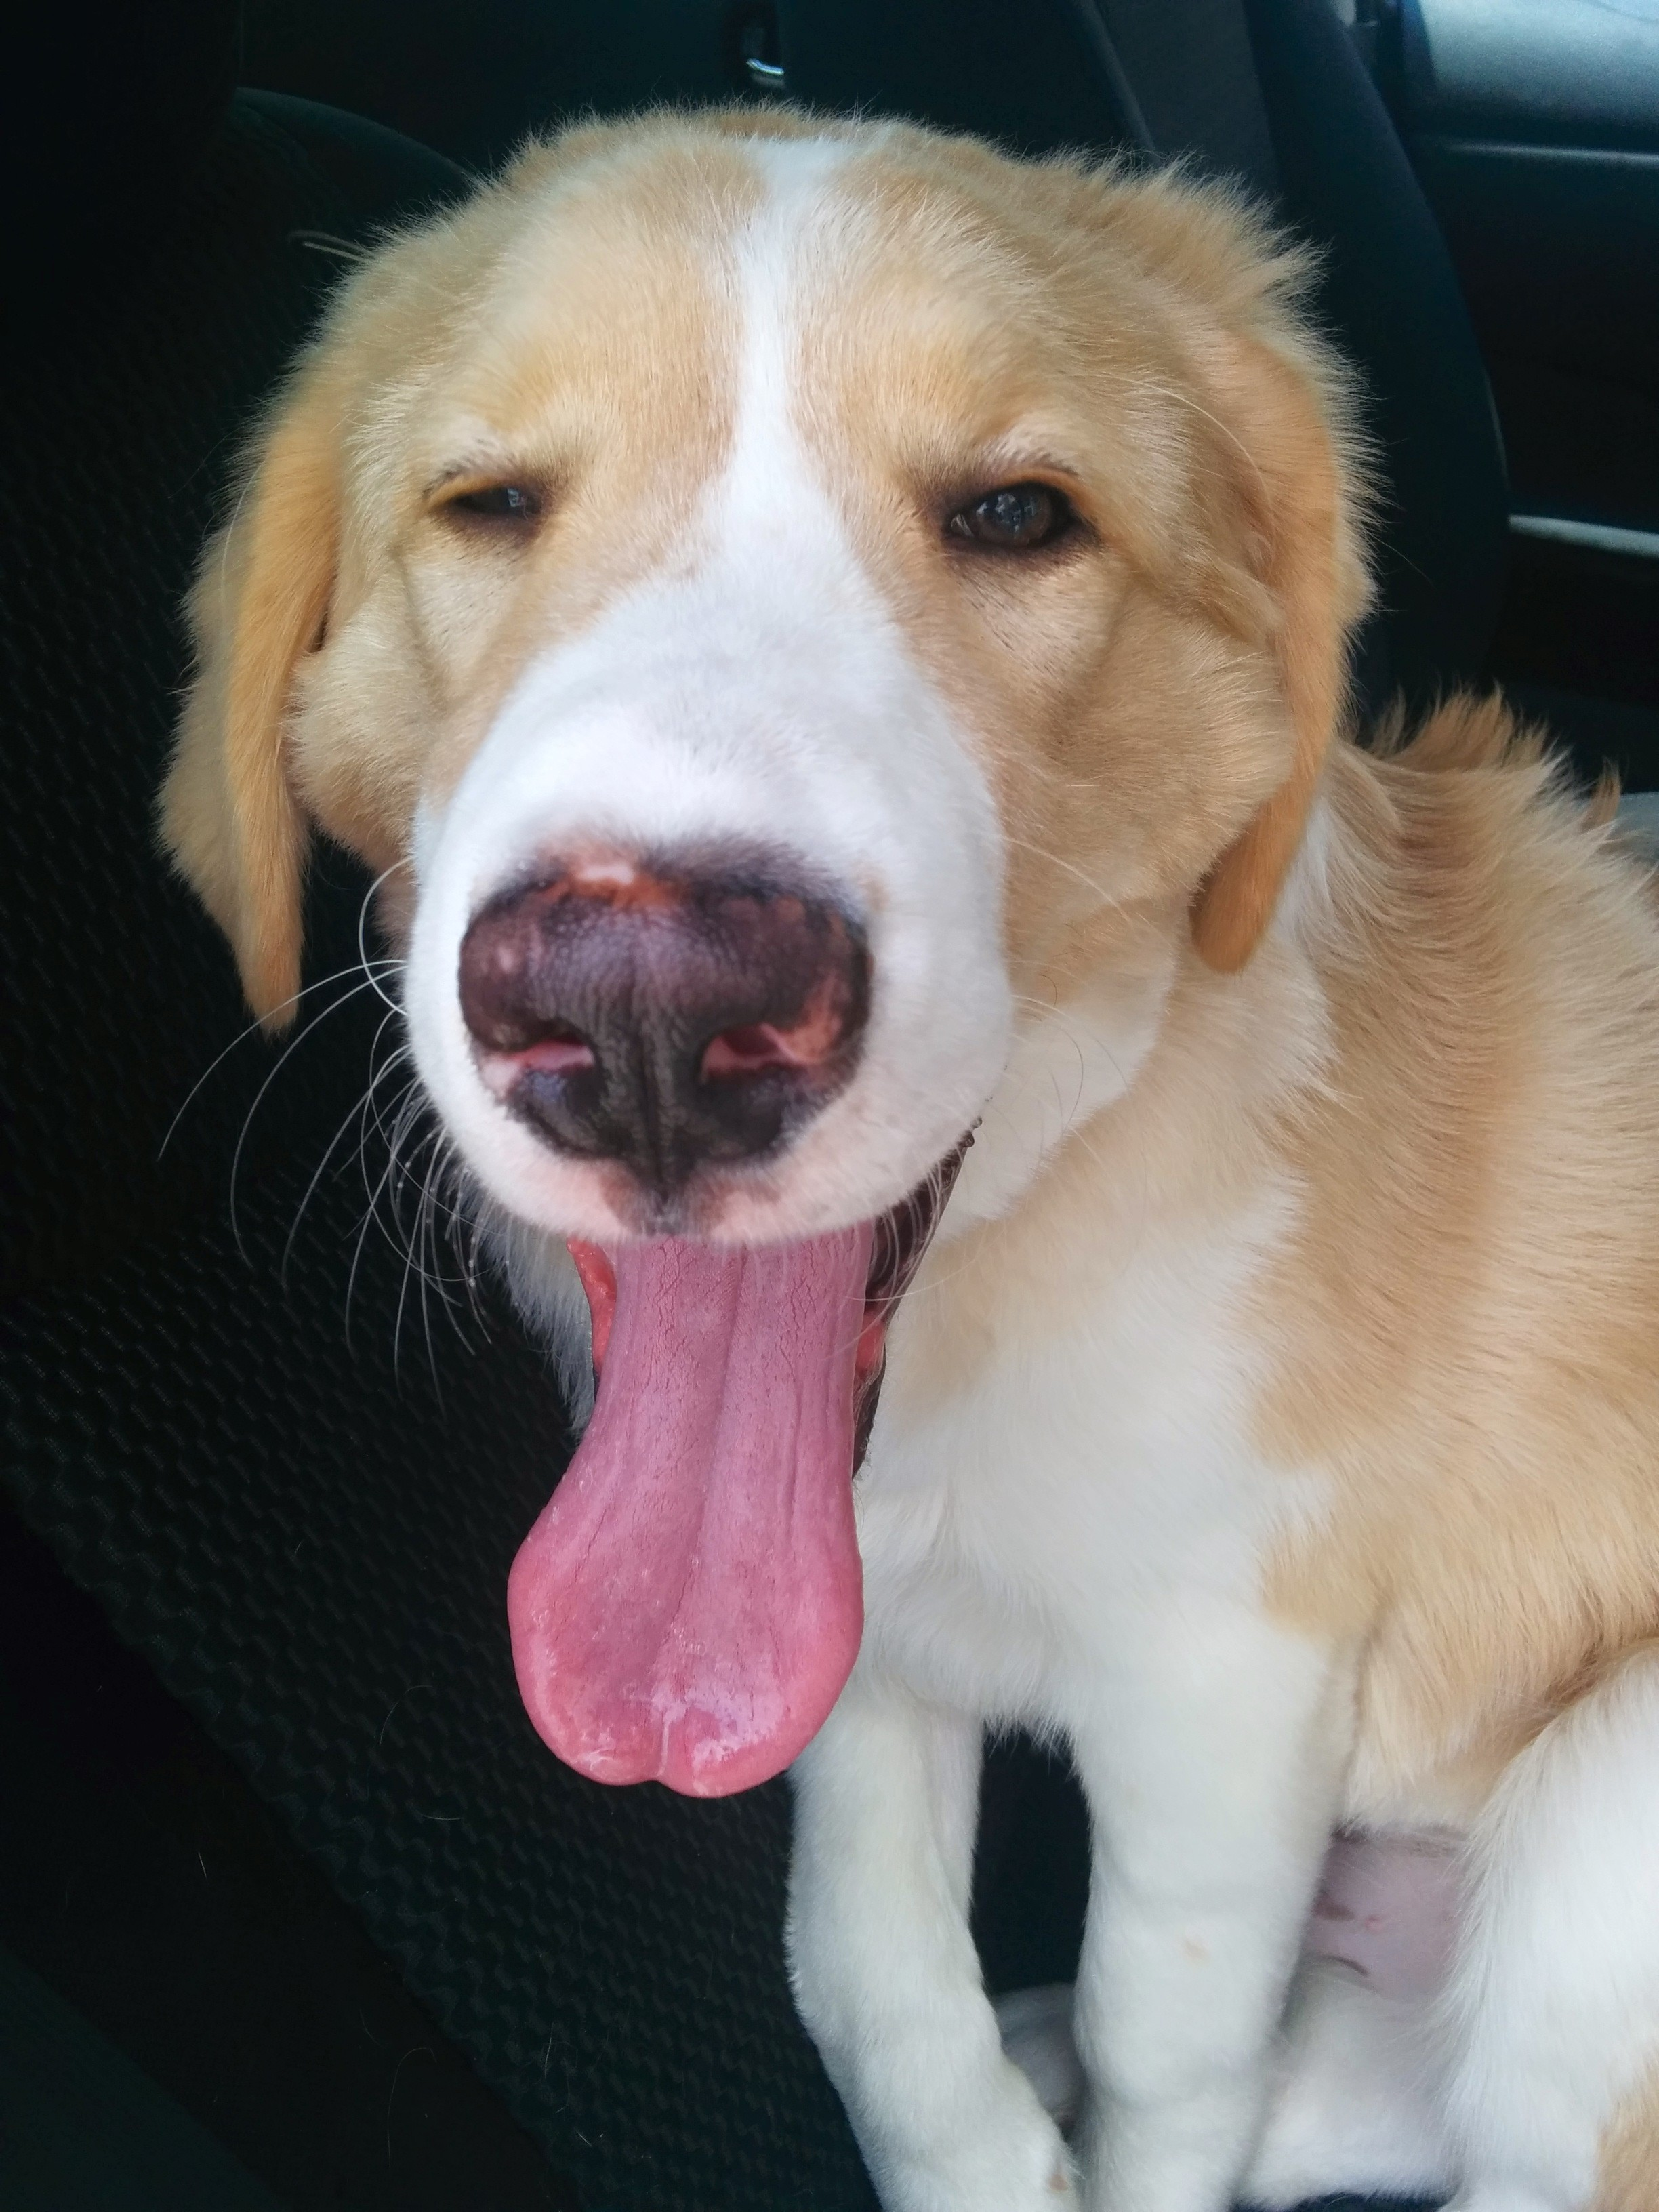
\includegraphics[width=.35\textwidth]{./images/max/totally_baked.jpg}
    \caption{Maxwell looking totally baked.}
    \label{fig:totally_baked}
\end{figure}

\begin{figure}[H]
    \centering
    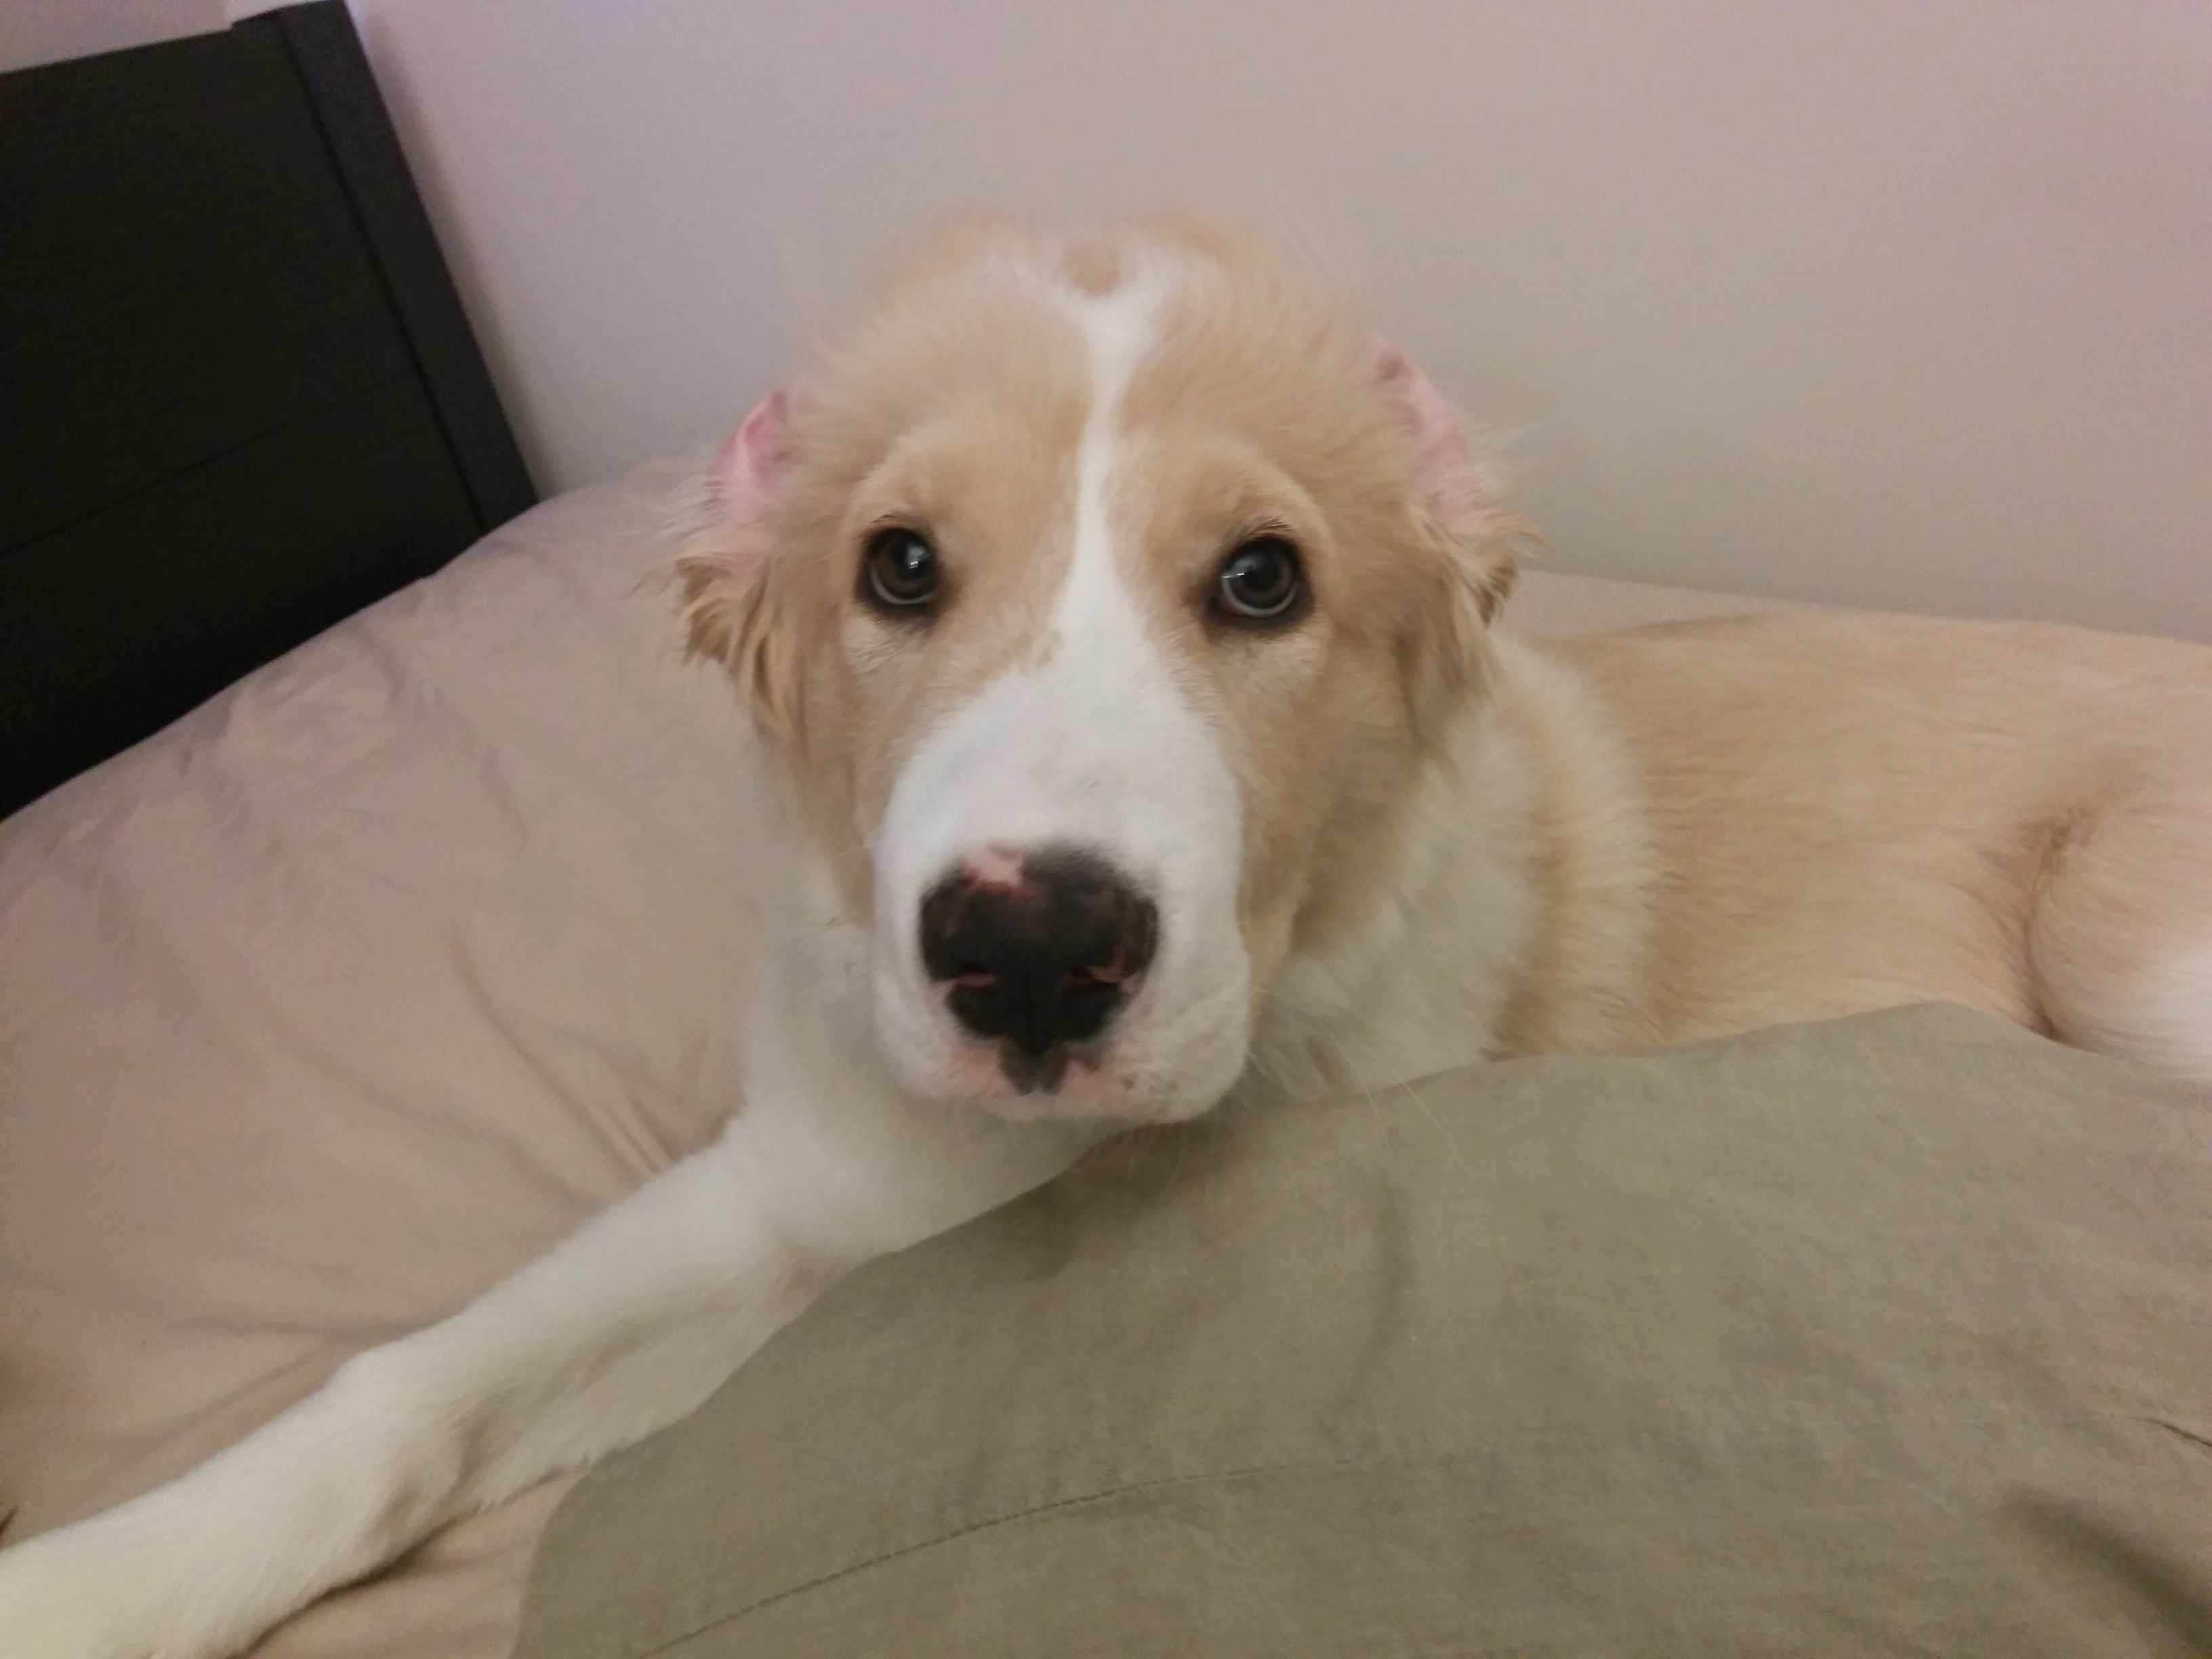
\includegraphics[width=.35\textwidth]{./images/max/natural_ears.jpg}
    \caption{Maxwell's ears in their natural position.}
    \label{fig:natural_ears}
\end{figure}

\begin{figure}[H]
    \centering
    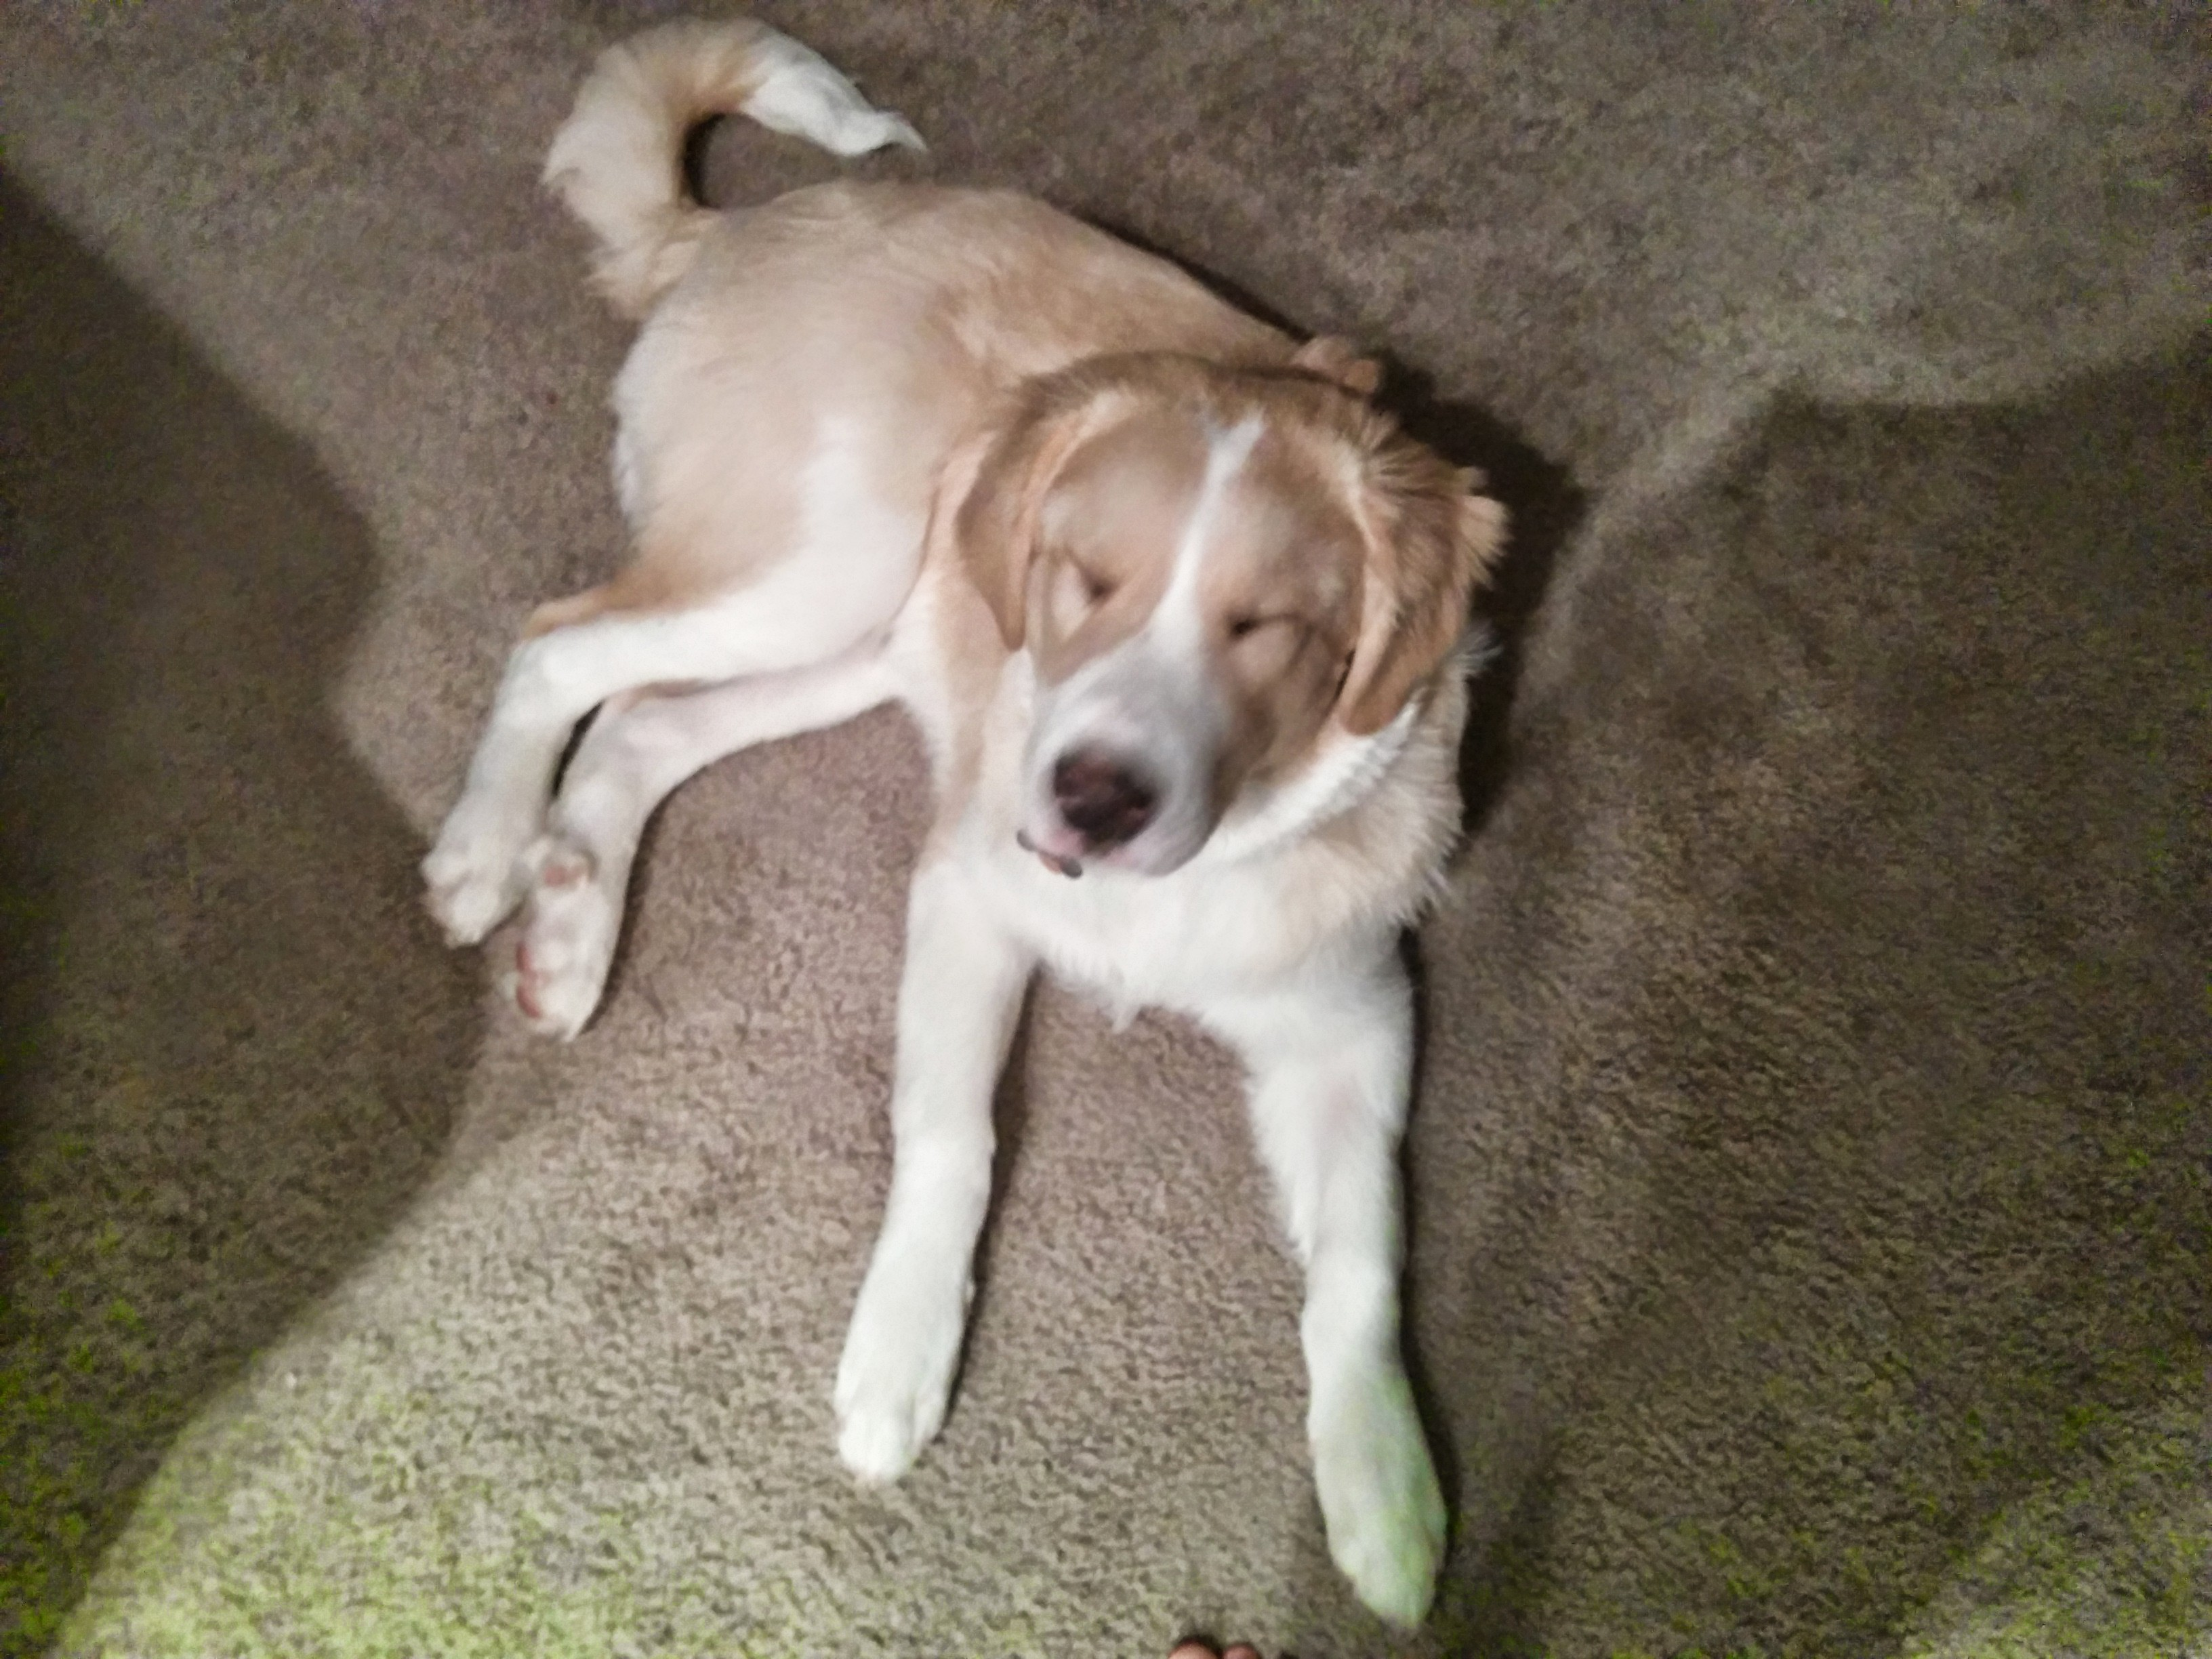
\includegraphics[width=.35\textwidth]{./images/max/goofball.jpg}
    \caption{Maxwell being a goofball.}
    \label{fig:goofball}
\end{figure}

\end{document}
